%%%%%%%%%%%%%%%%%%%%%%%%%%%%%%%%%%%%%%%%%
% Masters/Doctoral Thesis
% Mardown LaTeX Template
%
% Version 0.1 (05 Mar 2018)
%
% This template is based on a template pandoc's latex template and latex templates by:
% Vel (vel@latextemplates.com)
% Steve Gunn (http://users.ecs.soton.ac.uk/srg/softwaretools/document/templates/)
% Sunil Patel (http://www.sunilpatel.co.uk/thesis-template/)
%
% Template license:
% CC BY-NC-SA 3.0 (http://creativecommons.org/licenses/by-nc-sa/3.0/)
%
%%%%%%%%%%%%%%%%%%%%%%%%%%%%%%%%%%%%%%%%%

%----------------------------------------------------------------------------------------
%	PACKAGES AND OTHER DOCUMENT CONFIGURATIONS
%----------------------------------------------------------------------------------------

\PassOptionsToPackage{unicode=true}{hyperref} % options for packages loaded elsewhere
\PassOptionsToPackage{hyphens}{url}
\PassOptionsToPackage{dvipsnames,svgnames*,x11names*}{xcolor}

\documentclass[
11pt, % The default document font size, options: 10pt, 11pt, 12pt
%oneside, % Two side (alternating margins) for binding by default, uncomment to switch to one side
english, % ngerman for German
singlespacing, % Single line spacing, alternatives: onehalfspacing or doublespacing
%draft, % Uncomment to enable draft mode (no pictures, no links, overfull hboxes indicated)
%nolistspacing, % If the document is onehalfspacing or doublespacing, uncomment this to set spacing in lists to single
%liststotoc, % Uncomment to add the list of figures/tables/etc to the table of contents
%toctotoc, % Uncomment to add the main table of contents to the table of contents
%parskip, % Uncomment to add space between paragraphs
%nohyperref, % Uncomment to not load the hyperref package
headsepline, % Uncomment to get a line under the header
%chapterinoneline, % Uncomment to place the chapter title next to the number on one line
%consistentlayout, % Uncomment to change the layout of the declaration, abstract and acknowledgements pages to match the default layout
]{MastersDoctoralThesis} % The class file specifying the document structure

\usepackage[l2tabu, orthodox]{nag} % this is to make sure I use some modern LaTeX tactics

\usepackage{polyglossia}
\setdefaultlanguage[variant=uk]{english}
%\setotherlanguage{spanish}

\usepackage{lipsum}

%\usepackage{ifxetex,ifluatex}
\usepackage{fixltx2e} % provides \textsubscript

\usepackage{mathtools}
\usepackage{unicode-math}
\defaultfontfeatures{Ligatures=TeX,Scale=MatchLowercase}
\usepackage{fontspec}
\usepackage{xcolor}
%\usepackage{newpxtext,newpxmath} % Use the New PX font by default
% Font suggestion from: https://tex.stackexchange.com/a/50593
\setmainfont{texgyrepagella}[
  Extension=.otf,
  UprightFont=*-regular,
  ItalicFont=*-italic,
  BoldFont=*-bold,
  BoldItalicFont=*-bolditalic,
  Numbers=OldStyle,
]
%\setmonofont[Color=ForestGreen]{Fira Code}

\usepackage[backend=biber,natbib=false,style=apa]{biblatex}
\DeclareLanguageMapping{english}{english-apa}

\addbibresource{bibliography.bib} % The filename of the bibliography

\usepackage[autostyle=true]{csquotes} % Required to generate language-dependent quotes in the bibliography

%----------------------------------------------------------------------------------------
%	MARGIN SETTINGS
%----------------------------------------------------------------------------------------

\geometry{
	paper=letterpaper, % Change to letterpaper for US letter
  textwidth=165mm,
  textheight=225mm,
	%inner=2.5cm, % Inner margin
	%outer=3.8cm, % Outer margin
	bindingoffset=.5cm, % Binding offset
	%top=1.5cm, % Top margin
	%bottom=1.5cm, % Bottom margin
	%showframe, % Uncomment to show how the type block is set on the page
}

%----------------------------------------------------------------------------------------
%	THESIS INFORMATION
%----------------------------------------------------------------------------------------

\thesistitle{Static Analysis of Python Programs using Abstract Interpretation: An
Application to Tensor Shape Analysis} % Your thesis title, this is used in the title and abstract, print it elsewhere with \ttitle
\supervisor{PhD. Felipe \textsc{Restrepo Calle}} % Your supervisor's name, this is used in the title page, print it elsewhere with \supname
\cosupervisor{PhD. Fabio Augusto \textsc{González}} % \cosupname
\examiner{} % Your examiner's name, this is not currently used anywhere in the template, print it elsewhere with \examname
\degree{Masters Systems and Computer Engineering} % Your degree name, this is used in the title page and abstract, print it elsewhere with \degreename
\author{Elkin Alejandro \textsc{Cruz Camacho}} % Your name, this is used in the title page and abstract, print it elsewhere with \authorname
\addresses{} % Your address, this is not currently used anywhere in the template, print it elsewhere with \addressname

\subject{Systems and Computer Engineering} % Your subject area, this is not currently used anywhere in the template, print it elsewhere with \subjectname
\keywords{} % Keywords for your thesis, this is not currently used anywhere in the template, print it elsewhere with \keywordnames
\university{\href{https://www.unal.edu.co}{Universidad Nacional de Colombia}} % Your university's name and URL, this is used in the title page and abstract, print it elsewhere with \univname
\department{Departamento de Ingeniería de Sistemas e Industrial} % Your department's name and URL, this is used in the title page and abstract, print it elsewhere with \deptname
\group{PLaS - Mindlab} % Your research group's name and URL, this is used in the title page, print it elsewhere with \groupname
\faculty{\href{https://ingenieria.bogota.unal.edu.co}{Facultad de Ingeniería}} % Your faculty's name and URL, this is used in the title page and abstract, print it elsewhere with \facname

\AtBeginDocument{
\hypersetup{pdftitle=\ttitle} % Set the PDF's title to your title
\hypersetup{pdfauthor=\authorname} % Set the PDF's author to your name
\hypersetup{pdfkeywords=\keywordnames} % Set the PDF's keywords to your keywords
}

%%%% Copied from Pandoc's markdown

% use upquote if available, for straight quotes in verbatim environments
\IfFileExists{upquote.sty}{\usepackage{upquote}}{}
% use microtype if available
\IfFileExists{microtype.sty}{%
\usepackage[]{microtype}
\UseMicrotypeSet[protrusion]{basicmath} % disable protrusion for tt fonts
}{}

\usepackage{xcolor}
\usepackage{color}
\usepackage{fancyvrb}
\newcommand{\VerbBar}{|}
\newcommand{\VERB}{\Verb[commandchars=\\\{\}]}
\DefineVerbatimEnvironment{Highlighting}{Verbatim}{commandchars=\\\{\}}
% Add ',fontsize=\small' for more characters per line
\newenvironment{Shaded}{}{}
\newcommand{\AlertTok}[1]{\textcolor[rgb]{1.00,0.00,0.00}{\textbf{#1}}}
\newcommand{\AnnotationTok}[1]{\textcolor[rgb]{0.38,0.63,0.69}{\textbf{\textit{#1}}}}
\newcommand{\AttributeTok}[1]{\textcolor[rgb]{0.49,0.56,0.16}{#1}}
\newcommand{\BaseNTok}[1]{\textcolor[rgb]{0.25,0.63,0.44}{#1}}
\newcommand{\BuiltInTok}[1]{#1}
\newcommand{\CharTok}[1]{\textcolor[rgb]{0.25,0.44,0.63}{#1}}
\newcommand{\CommentTok}[1]{\textcolor[rgb]{0.38,0.63,0.69}{\textit{#1}}}
\newcommand{\CommentVarTok}[1]{\textcolor[rgb]{0.38,0.63,0.69}{\textbf{\textit{#1}}}}
\newcommand{\ConstantTok}[1]{\textcolor[rgb]{0.53,0.00,0.00}{#1}}
\newcommand{\ControlFlowTok}[1]{\textcolor[rgb]{0.00,0.44,0.13}{\textbf{#1}}}
\newcommand{\DataTypeTok}[1]{\textcolor[rgb]{0.56,0.13,0.00}{#1}}
\newcommand{\DecValTok}[1]{\textcolor[rgb]{0.25,0.63,0.44}{#1}}
\newcommand{\DocumentationTok}[1]{\textcolor[rgb]{0.73,0.13,0.13}{\textit{#1}}}
\newcommand{\ErrorTok}[1]{\textcolor[rgb]{1.00,0.00,0.00}{\textbf{#1}}}
\newcommand{\ExtensionTok}[1]{#1}
\newcommand{\FloatTok}[1]{\textcolor[rgb]{0.25,0.63,0.44}{#1}}
\newcommand{\FunctionTok}[1]{\textcolor[rgb]{0.02,0.16,0.49}{#1}}
\newcommand{\ImportTok}[1]{#1}
\newcommand{\InformationTok}[1]{\textcolor[rgb]{0.38,0.63,0.69}{\textbf{\textit{#1}}}}
\newcommand{\KeywordTok}[1]{\textcolor[rgb]{0.00,0.44,0.13}{\textbf{#1}}}
\newcommand{\NormalTok}[1]{#1}
\newcommand{\OperatorTok}[1]{\textcolor[rgb]{0.40,0.40,0.40}{#1}}
\newcommand{\OtherTok}[1]{\textcolor[rgb]{0.00,0.44,0.13}{#1}}
\newcommand{\PreprocessorTok}[1]{\textcolor[rgb]{0.74,0.48,0.00}{#1}}
\newcommand{\RegionMarkerTok}[1]{#1}
\newcommand{\SpecialCharTok}[1]{\textcolor[rgb]{0.25,0.44,0.63}{#1}}
\newcommand{\SpecialStringTok}[1]{\textcolor[rgb]{0.73,0.40,0.53}{#1}}
\newcommand{\StringTok}[1]{\textcolor[rgb]{0.25,0.44,0.63}{#1}}
\newcommand{\VariableTok}[1]{\textcolor[rgb]{0.10,0.09,0.49}{#1}}
\newcommand{\VerbatimStringTok}[1]{\textcolor[rgb]{0.25,0.44,0.63}{#1}}
\newcommand{\WarningTok}[1]{\textcolor[rgb]{0.38,0.63,0.69}{\textbf{\textit{#1}}}}

\usepackage{graphicx,grffile}
\makeatletter
\def\maxwidth{\ifdim\Gin@nat@width>\linewidth\linewidth\else\Gin@nat@width\fi}
\def\maxheight{\ifdim\Gin@nat@height>\textheight\textheight\else\Gin@nat@height\fi}
\makeatother
% Scale images if necessary, so that they will not overflow the page
% margins by default, and it is still possible to overwrite the defaults
% using explicit options in \includegraphics[width, height, ...]{}
\setkeys{Gin}{width=\maxwidth,height=\maxheight,keepaspectratio}
\setlength{\emergencystretch}{3em}  % prevent overfull lines
\providecommand{\tightlist}{%
  \setlength{\itemsep}{0pt}\setlength{\parskip}{0pt}}
% Redefines (sub)paragraphs to behave more like sections
\ifx\paragraph\undefined\else
\let\oldparagraph\paragraph
\renewcommand{\paragraph}[1]{\oldparagraph{#1}\mbox{}}
\fi
\ifx\subparagraph\undefined\else
\let\oldsubparagraph\subparagraph
\renewcommand{\subparagraph}[1]{\oldsubparagraph{#1}\mbox{}}
\fi

% set default figure placement to htbp
\makeatletter
\def\fps@figure{htbp}
\makeatother

%%% Other little tweaks

% Based on: https://tex.stackexchange.com/a/17819
\newif\ifdraft
\drafttrue

% TODONOTES
\ifdraft
\usepackage[textsize=tiny,bordercolor=yellow,color=yellow,textwidth=4cm,colorinlistoftodos]{todonotes}
\else
\usepackage[disable]{todonotes}
\fi

% Addittional information passed by the user
%\usepackage{graphicx}

%\usepackage{layout} % package to look at the page layout

%\hypersetup{bookmarks=true,
%            pdfauthor={},
%            colorlinks=true,
%            citecolor=blue,
%            urlcolor=blue,
%            linkcolor=magenta}

\usepackage{setspace} % for pandoc-citeproc-preamble

%%%% todonotes stuff %%%%
\newcommand{\inlinetodo}[1]{\todo[inline,size=\normalsize]{#1}}

% Custom color todos: https://tex.stackexchange.com/a/178806
\usepackage{xargs} % Use more than one optional parameter in a new commands
\newcommandx{\change}[2][1=]{\todo[linecolor=red,backgroundcolor=red!25,bordercolor=red,#1]{#2}}
\newcommandx{\ichange}[2][1=]{\todo[inline,linecolor=red,backgroundcolor=red!25,bordercolor=red,#1]{#2}}

\newcommand{\nonsection}[1]{\vspace{3mm}\noindent\textbf{\large #1}\vspace{2mm}}

% color for "monospace" inline text
%\usepackage{xcolor}
%\usepackage{soulutf8}
\usepackage[normalem]{ulem} % use normalem to protect \emph
\newcommand\hl{\bgroup\markoverwith
  {\textcolor{yellow}{\rule[-.5ex]{2pt}{2.5ex}}}\ULon}

\begin{document}

\frontmatter % Use roman page numbering style (i, ii, iii, iv...) for the pre-content pages

\pagestyle{plain} % Default to the plain heading style until the thesis style is called for the body content

%----------------------------------------------------------------------------------------
%	TITLE PAGE
%----------------------------------------------------------------------------------------

\begin{titlepage}
\begin{center}

\vspace*{.06\textheight}

\includegraphics[width=0.23\textwidth]{figures/escudo.png}\\
{\scshape\LARGE \univname\par}\vspace{1.2cm} % University name
\textsc{\Large Master thesis}\\[0.3cm] % Thesis type

\HRule \\[0.4cm] % Horizontal line
{\huge \bfseries \ttitle\par}\vspace{0.4cm} % Thesis title
\HRule \\[8mm] % Horizontal line

\begin{minipage}[t]{0.4\textwidth}
\begin{flushleft} \large
\emph{Author:}\\
\authorname
\end{flushleft}
\end{minipage}
\begin{minipage}[t]{0.4\textwidth}
\begin{flushright} \large
\emph{Supervisor:} \\
\supname
\\[2mm]
\emph{Co-supervisor:} \\
\cosupname

\end{flushright}
\end{minipage}\\[8mm]

\vfill

\large \textit{
  A thesis submitted in fulfillment of the requirements\\ for the degree of \degreename%
}\\[0.3cm] % University requirement text
\textit{in the}\\[0.4cm]
\groupname\\%
\deptname\\[1.3cm] % Research group name and department name

\vfill

{\large \today}\\[8mm] % Date
%\includegraphics{Logo} % University/department logo - uncomment to place it

\vfill
\end{center}
\end{titlepage}


\cleardoublepage

%----------------------------------------------------------------------------------------
%	QUOTATION PAGE
%----------------------------------------------------------------------------------------

\vspace*{0.2\textheight}

\noindent\enquote{\itshape The truth is that everyone is bored, and devotes himself to
cultivating habits.}\bigbreak

\hfill Albert Camus, The Plague

\vspace{2cm}

\noindent\enquote{\itshape Perhaps I'm old and tired, but I think that the chances of
finding out what's actually going on are so absurdly remote that the only thing to do
is to say, "Hang the sense of it," and keep yourself busy.}\bigbreak

\hfill Douglas Adams, The Hitchhiker's Guide to the Galaxy


%----------------------------------------------------------------------------------------
%	ABSTRACT PAGE
%----------------------------------------------------------------------------------------

\begin{abstractpage}
% \begin{abstract}[Resumen][spanish]
% {\inlinetodo{Translate from Abstract}}
% \end{abstract}

\begin{abstract}[Abstract][english]
Tensors are, an extension of arrays, widely used in a variety of
programming tasks. Tensors are the building block of many modern machine
learning frameworks and are fundamental in the definition of deep
learning models. Linters are indispensable tools for today's developers,
as they help the developers to check code before executing it. Despite
the popularity of tensors, linters for Python that check and flag code
with tensors are nonexistent. Given the tremendous amount of work done
in Python with (and without) tensors, it is quite baffling that little
work has been done in this regard. Abstract Interpretation is a
methodology/framework for statically analysing code. The idea of
Abstract Interpretation is to soundly overapproximate the result of
running a piece of code over all possible inputs of the program. A sound
overapproximation ensures that the Abstract Interpreter will never omit
a true negative, i.e.~if a piece of code is not flagged by the Abstract
Interpreter, then it can be safely assumed that the code will not fail.
The Abstract Interpreter can be modified so that it only outputs true
positives, although losing soundness, i.e.~the interpreter can flag
which parts of the code are going to fail no matter how the code is run.

In this work, we formalise a subset of Python with emphasis on tensor
operations. Our formal Python semantics are based on The Python Language
Reference. An Abstract Interpreter was defined and implemented from the
Python formalisation. We show how each part of the Abstract Interpreter
was built: the Abstract Domains defined, and the inferred formal
semantics. We present the structure of Pytropos, the Abstract
Interpreter implemeted. Pytropos is able to check NumPy array operations
taking into account broadcasting and complex NumPy functions as
\texttt{array} and \texttt{dot}. We constructed 80 unit test cases
checking the capabilities of Pytropos and 50 property test cases
checking compliance with the official Python implementation. We show
what and how many bugs the Abstract Interpreter was able to find.
\end{abstract}
\end{abstractpage}

%----------------------------------------------------------------------------------------
%	ACKNOWLEDGEMENTS
%----------------------------------------------------------------------------------------

\begin{acknowledgements}
\addchaptertocentry{\acknowledgementname} % Add the acknowledgements to the table of contents
{\inlinetodo{fill me!!! I am the acknowledgements}}
\end{acknowledgements}

%----------------------------------------------------------------------------------------
%	LIST OF CONTENTS/FIGURES/TABLES PAGES
%----------------------------------------------------------------------------------------

\tableofcontents % Prints the main table of contents

 % Prints the list of figures

 % Prints the list of tables


%----------------------------------------------------------------------------------------
%	DEDICATION
%----------------------------------------------------------------------------------------

\dedicatory{{\inlinetodo{fill me!!! I am the dedication}}}

%----------------------------------------------------------------------------------------
%	THESIS CONTENT - CHAPTERS
%----------------------------------------------------------------------------------------

\mainmatter % Begin numeric (1,2,3...) page numbering

\pagestyle{thesis} % Return the page headers back to the "thesis" style

% Include the chapters of the thesis as separate files from the Chapters folder
% Uncomment the lines as you write the chapters

\listoftodos

\newpage

\hypertarget{prelude}{%
\chapter*{Prelude}\label{prelude}}
\addcontentsline{toc}{chapter}{Prelude}

Dear reader, thank you for picking this thesis to read. Reading a thesis
is often an annoying \emph{task}, and it is also a very difficult task
to do as well. Despite what my advisors tell me, I like to write in a
style slightly different from the style seen often in science
publications. I ask you, dear reader, to tolerate my style of writing, I
try to write the text as if I were explaining all the stuff to my
past-self (one and a half years in the past). You will find many
overexplanatory sentences, paragraphs and complete subchapters, with
examples and other uncommon customs. My intention is, after all, to be a
guide for my past-self to come where I have arrived, but faster.

\hypertarget{introduction}{%
\chapter{Introduction}\label{introduction}}

\hypertarget{motivation}{%
\section{Motivation}\label{motivation}}

Dynamically typed programming languages, like Python and Ruby, have been
rising in popularity over the last two decades. Their simple syntax,
ease of use, out-of-the-box REPL\footnote{Read-eval-print loop}, and the
great number of libraries they come bundled up with have been all
factors to their rise. Indeed, being able to write and execute code on
the fly makes for very speedy development cycles, especially at the
initial stages of development. Howeverwarranting that code written in
these kinds of languages is not an easy task, as most efforts on
verification and static analysis, in general, have been targeted towards
the needs of statically typed programming languages.

Dynamically typed programming languages, such as Python
\autocite{van2007python}, only check for type mismatches at runtime,
i.e.~errors between variable types get only detected when the code is
run. For example, consider the following piece of Python code:

\begin{Shaded}
\begin{Highlighting}[]
\NormalTok{myvar }\OperatorTok{=} \StringTok{"Some text in a string"}
\NormalTok{other }\OperatorTok{=} \FloatTok{4.1}
\NormalTok{result }\OperatorTok{=} \StringTok{"oh my"} \OperatorTok{+} \DecValTok{2}  \CommentTok{# This will fail}
\BuiltInTok{print}\NormalTok{(result }\OperatorTok{+}\NormalTok{ other, myvar)}
\end{Highlighting}
\end{Shaded}

The code is syntactically correct but it fails to execute. Python will
interpret the first two lines and will be stuck at the third, where it
will throw an exception due to the fact that a string and a number
cannot be added up together.

A Static Type Analysis tool, such as MyPy \autocite{lehtosalo2016mypy},
is able to detect many type mismatches without ever running the code.
Mypy has the ability to infer the type of variables, e.g., it detects
that \texttt{other} is of type \texttt{float} and \texttt{myvar} of type
\texttt{str}. Python dynamic nature makes it extraordinarily hard to
statically analyse, in fact, due to Python introspection capabilities it
is impossible to ever warranty anything about a piece of Python code
without assuming some basic behaviour by the interpreter. Mypy tackles
the undecidability problem of Python dynamic nature by restricting the
number of valid Python programs to those that conform to a static type
system\footnote{I will like to express my inmense gratitude to the MyPy
  team for letting me save time by writing a tool that can detect faulty
  code. I do not know how many hours they saved me from endless
  frustration at debugging Python code. What I like more about MyPy is
  that writing code with it feels just remarkably similar to writing
  code in language with stronger static type systems such as Haskell.
  Thank you, Lehtosalo, Guido, and the whole crew behind MyPy!}.

Even with some assumptions in place, Mypy's inference ability only goes
so far as to infer the type of variables but not of functions. Mypy
allows, optionally, to add type annotations to the code (to either
variables or functions). Type annotations allow more (restrictive and)
precise types, which help Mypy to catch more potential bugs.

However useful Mypy is, its assumptions limit it from a whole chunk of
valid and correct Python code\footnote{For example, there is no way
  (currently) to make MyPy happy about the function
  \texttt{def\ addtwice(x,\ y):\ return\ x\ +\ y\ +\ y;\ addtwice(3,2);\ addtwice(\textquotesingle{}a\textquotesingle{},\textquotesingle{}b\textquotesingle{})}.
  If no type annotations is given, MyPy alerts the user on the usage of
  non-typed functions. But no type can satisfy the assertion because of
  the \enquote{polymorphisity} of the \texttt{+} operation.}. There are
many scenarios where even with type annotations Mypy cannot detect a bug
in the code. For example, consider the following piece of python
code\footnote{Notice the lack of type annotations in this example. Mypy
  is able to infer the type of the variables in this example, and it
  makes no difference to annotate the variables with their types
  (everything in Python is an object, then the type of any variable
  above is the class from which it is instantiated)}:

\begin{Shaded}
\begin{Highlighting}[]
\ImportTok{import}\NormalTok{ numpy }\ImportTok{as}\NormalTok{ np}
\NormalTok{x }\OperatorTok{=}\NormalTok{ np.array( [[}\DecValTok{1}\NormalTok{,}\DecValTok{2}\NormalTok{,}\DecValTok{3}\NormalTok{], [}\DecValTok{4}\NormalTok{,}\DecValTok{5}\NormalTok{,}\DecValTok{6}\NormalTok{]] ) }\CommentTok{# shape (2,3)}
\NormalTok{y }\OperatorTok{=}\NormalTok{ np.array( [[}\DecValTok{7}\NormalTok{], [}\DecValTok{0}\NormalTok{], [}\DecValTok{2}\NormalTok{], [}\DecValTok{1}\NormalTok{]] ) }\CommentTok{# shape (4,1)}
\NormalTok{z }\OperatorTok{=}\NormalTok{ np.dot( x, y ) }\CommentTok{# trying to apply dot product}
\end{Highlighting}
\end{Shaded}

We are using in this example a well known Python library, NumPy
\autocite{oliphant2006guide}, but it could have been, just as well,
TensorFlow \autocite{abadi_tensorflow_2016} or any other library with
support for tensors and tensor operators. Tensors are a generalization
of vectors and arrays. A vector of size \texttt{n}, or array of shape
\texttt{(n,)}, contains exactly \(n\) elements; a matrix of size
\(n \times m\), alternatively, a matrix of shape \texttt{(n,\ m)}, is a
structure that holds \(n \cdot m\) elements; and, a tensor is a
structure that can have any integer tuple as its shape, e.g.,
\texttt{(2,\ 5,\ 6)} which could hold \(2 \cdot 5 \cdot 6 = 60\)
elements.

The example above will fail to run completely as it hits an erroneous
condition at the last line. Two arrays/tensors are created, \texttt{x}
and \texttt{y} with shapes \texttt{(2,\ 3)} and \texttt{(4,\ 1)},
respectively, then a matrix multiplication with both tensors tries to be
performed, but it fails because the shapes of the two matrices are
incompatible (\(3\ne4\)). The call to \texttt{np.dot} fails, but we
won't know this until we execute the code. To summarise, the code above
type checks in MyPy even though it fails to run.

If it were possible to add the shape of the tensors as part of the type
definitions, we could potentially type check for mismatches of tensor's
shapes. Unfortunately, there does not seem to be a straightforward way
to add the shape of tensors to types and check them in MyPy.

Tensors allow writing computations more concisely. Tensor operations are
also highly optimisable and can be run in parallel. With the advent of
Deep Learning in every possible realm in which it can be applied,
tensors have become more of a central figure in developers toolkit.
Tensor operations fail if the tensors are not of the right shape. To
statically analyse if operations between tensors are valid, one needs to
calculate the shape of tensors which requires to statically analyse the
value of variables in the language (also called, Static Value Analysis).

\hypertarget{problem-definition}{%
\section{Problem Definition}\label{problem-definition}}

Tensors are becoming an essential abstraction in the toolkit of
developers. Tools tailored to work with or based on tensors have been
popping out in recent years. It is therefore imperative to develop
analysis tools to verify and flag potential bugs. A Static Value
Analysis tool focused on tensor shape analysis could aid developers in
their work, as it could be able to flag potential bugs related to the
shapes of tensors as the developer writes code.

All of the theoretical approaches that tackle the problem focus on type
checking tensors and tensor operations. \textcite{griffioen_type_2015},
\textcite{slepak_array-oriented_2014}, and \textcite{rink_modeling_2018}
define a type system extended with tensors and tensor operations. The
principal idea of these type systems is to encode the restrictions that
the operations on tensors require, a tensor operation is valid if the
restriction checks with the tensors.

Practical attempts have been mainly focused on languages with strong
type systems, and recently some in Python
\autocites{fromherz_static_2018}{monat_static_2018}.
\textcite{chen_typesafe_2017} (in Scala) and
\textcite{eaton_statically_2006} (in Haskell) have tried to annotate
tensors' types with their shapes, leaving the compiler's type check
inference system to check the shapes. At the time
\textcite{eaton_statically_2006} proposed his methodology to extend
types with additional data, GHC (Glasgow Haskell Compiler), the by
default Haskell compiler, didn't have many capabilities to work with
data at the type level, resulting in some rather complicated code to
read and write. A recent approach to type check tensors in Haskell has
been shown in a library written by \textcite{elkin_haskell_2018}, which
uses the updated Dependent Type System of Haskell to code and enforce
type shapes.

Abstract Interpretation is a framework for static analysis. The main
idea of Abstract Interpretation is to overapproximate the result of
computing a piece of code. Any piece of code can be run in an Abstract
Interpreter, an interpreter build from the semantics defined by Abstract
Interpretation, in a finite amount of time. To warranty that the
Abstract Interpreter runs in a finite amount of time, Abstract
Interpretation defines a series of rules that force to overapproximate
the result of executing operations by the program. Abstract
Interpretation is especially useful for Static Value Analysis as the
rules to derive the semantics of an Abstract Interpreter from the formal
semantics of the language are very well studied, formalised and explicit
\autocite{cousot_abstract_1977}.

Writing an Abstract Interpreter for Python requires the formal semantics
of Python as a starting point. Unfortunately, Python does not have any
official formal semantics defined. Some attempts to define a formal
semantics for Python have been done
\autocites{politz_python_2013}{fromherz_static_2018}{guth_formal_2013}{ranson_semantics_2008}
but none of them take into account type annotations.

\textbf{Problem:} Building an Abstract Interpreter for Python to
Statically Value-Analyse tensor operations.

{\inlinetodo{Should I add some research questions?}}

\hypertarget{assumptions-and-scope}{%
\subsubsection{Assumptions and Scope}\label{assumptions-and-scope}}

Very little can be asserted from a piece of code in a programming
language like Python without making any assumptions about the
environment. For example, consider the following piece of code:

\begin{Shaded}
\begin{Highlighting}[]
\CommentTok{# runme.py}
\NormalTok{a }\OperatorTok{=} \BuiltInTok{int}\NormalTok{(}\StringTok{'6'}\NormalTok{) }\OperatorTok{+} \DecValTok{2}
\BuiltInTok{print}\NormalTok{(}\DecValTok{7}\NormalTok{)}
\ControlFlowTok{assert}\NormalTok{ a }\OperatorTok{==} \DecValTok{8}
\end{Highlighting}
\end{Shaded}

One may be tempted to say that the code above never fails, but it would
be mistaken. Thanks to Python's introspection capabilities, the code
above could do just about anything. A piece of Python code can be run
directly in the interpreter or executed by an \VERB|\BuiltInTok{exec}|
or \VERB|\BuiltInTok{eval}| statement. The functions \texttt{int} and
\texttt{print} can be redefined to compute anything we want. For
example, consider the following piece of code in that calls
\texttt{runme.py}:

\begin{Shaded}
\begin{Highlighting}[]
\NormalTok{runme }\OperatorTok{=} \BuiltInTok{open}\NormalTok{(}\StringTok{'runme.py'}\NormalTok{).read()}
\NormalTok{fakeinit }\OperatorTok{=} \StringTok{"""}
\StringTok{def int(val):}
\StringTok{  return 3.0}
\StringTok{def print(val):}
\StringTok{  global a}
\StringTok{  a = val}
\StringTok{"""}
\BuiltInTok{exec}\NormalTok{(fakeinit }\OperatorTok{+}\NormalTok{ runme, \{\})  }\CommentTok{# Throws an exception}
\end{Highlighting}
\end{Shaded}

From now on, we will assume that any piece of code written in Python
will be called from the interpreter directly without changing the
behaviour of any builtin function or variable (this includes the
behaviour of variables and functions from non-builtin libraries as
NumPy), i.e.~we assume that the code will never be run by an
\VERB|\BuiltInTok{exec}| call but always \texttt{import}ed or
interpreted directly by \texttt{python\ file-code.py}.

As a developer, I can say that I like when I see a piece of code flag
wrong and IT IS really WRONG, but I despise when the opposite happens.
It is very annoying to have a tool flag every sentence you write as
wrong even though the code works just fine. We will assume from here
onwards that we want the Tensor Analysis to flag only errors that are
going to happen if the code is run, i.e.~we want only true positives not
maybe positives (as a lack of a better word).

Although, TensorFlow \autocite{abadi_tensorflow_2016}, PyTorch
\autocite{paszke2017pytorch} and other libraries would benefit from the
development of a tool targeted to check them, I chose to check NumPy's
tensor operations. NumPy is the standard library for computing with
tensors and it is used as backend on most projects.

Implementing an Abstract Interpreter, or any Static Analysis, for a
language like Python is a considerable undertaking, mainly because of
the breadth of characteristics a mature Programming Language like Python
has. Thus, we will centre on just a couple of Python core
characteristics and will leave others for future work. The
characteristics explored in the current document are:

\begin{itemize}
\tightlist
\item
  Builtin primitive variables: \texttt{int}, \texttt{float},
  \texttt{bool}, \texttt{None}, \texttt{list}, \texttt{tuple}
\item
  Primitive functions: \texttt{int}, \texttt{print}, \texttt{input},
  \ldots{}
\item
  Boolean and numeric operations: \texttt{+}, \texttt{-}, \texttt{*},
  \texttt{/}, \texttt{\%}, \texttt{**}, \texttt{\textless{}\textless{}},
  \texttt{\textgreater{}\textgreater{}}, \texttt{//},
  \texttt{\textless{}}, \texttt{\textless{}=}, \texttt{\textgreater{}}
  and \texttt{\textgreater{}=}
\item
  \texttt{if} and \texttt{while} staments
\item
  Import statement (limited only to the \texttt{numpy} library)
\item
  NumPy arrays and some of its methods/functions to work with NumPy
  arrays (including \texttt{dot}, \texttt{zeros}, \texttt{shape}, and
  numeric operations with broadcasting)
\end{itemize}

Consider the following piece of code:

\begin{verbatim}
if someval:
  i = 3
else:
  i = "ntr"
print(i)
\end{verbatim}

The variable \texttt{i} can be either an \texttt{int} or a \texttt{str},
thus the type of \texttt{i} should be \texttt{Union{[}int,str{]}}. If
the type of a variable is an \texttt{Union} type then we need to build
an Abstract Interpreter (actually, an Abstract Domain) aware of unions.
Building an Abstract Interpreter aware of \texttt{Union} types is not
considered part of this work, therefore if a variable holds more than
one value, e.g., it is either a \texttt{5} or \texttt{2.3}, then the
variable's type will be \texttt{Any} and not \texttt{Union}.
\texttt{Any} and \texttt{Union} types are defined in the \texttt{typing}
library \autocite{pep484}, an implementation of Gradual Typing\footnote{Gradual
  Typing is a kind of Static Type Analysis targeted to Dynamically Typed
  Languages like Python}.

Gradual Typing restricts the number of valid programs to those that type
check. A variable in Gradual Typing is of a specific type and it never
changes, i.e.~if a variable's type is set to be \texttt{int} then it can
only contain \texttt{int}s. \texttt{Union} types are meant to indicate
that a variable may take more than one value at any point in time, which
would mean that any variable with a \texttt{Union} type would
automatically become an \texttt{Any} in this work, but that is not the
truth. Consider the following piece of code:

\begin{verbatim}
i = 3
i = "ntr"
i += "ueor"
print(i)  # the type of `i` is `str`
\end{verbatim}

Under Gradual Typing, the type of \texttt{i} is
\texttt{Union{[}int,str{]}}, but we know that the variable \texttt{i}
holds only one type at \textbf{all} times, i.e. \texttt{i} never holds
two or more values as in the previous example. An Abstract Interpreter
would run each line sequentially, and it would never find a that the
value of \texttt{i} is both \texttt{int} and \texttt{str} at the same
time, i.e.~the variable is never considered to be of type \texttt{Any}
but it will have type \texttt{int} and then type \texttt{str} as the
code is run. In this regard, an Abstract Interpreter can give a better
approximation of what the types of a variable are at any point in time,
while Gradual Typing considers all possible types a variable may have at
any point in time.

To recapitulate, the assumptions and scope of the thesis are:

\begin{itemize}
\tightlist
\item
  The behaviour of builtins and imported variables and functions is
  always the same and is determined by the Python reference manual or
  the library's author, e.g., \texttt{input} is a function that returns
  a \texttt{str}.
\item
  The user will only be reported errors that will happen but no errors
  that \emph{may} happen (This means, the resulting tool is not a
  verification tool).
\item
  The Static Value Analysis centres around checking operations from the
  NumPy library.
\item
  Only a selected subset of Python characteristics and functions are
  explored.
\item
  A variable can hold only one type of value at the time. If a variable
  is set to hold values of different types at the same time, then its
  value will be \texttt{Any}.
\end{itemize}

\hypertarget{objectives}{%
\section{Objectives}\label{objectives}}

\hypertarget{general-objective}{%
\subsection{General objective}\label{general-objective}}

To design and implement a strategy for statically analyse tensor shapes
in Python to support early detection of potential bugs before execution.

\hypertarget{specific-objectives}{%
\subsection{Specific objectives}\label{specific-objectives}}

\begin{enumerate}
\def\labelenumi{\arabic{enumi}.}
\tightlist
\item
  To design and implement an abstract interpreter for Python.
\item
  To design and implement a strategy that uses the abstract interpreter
  to analyse the shapes of tensors for Python code.
\item
  To implement a tool that flags the bugs inferred by the abstract
  interprete.
\item
  To empirically evaluate the developed static analysis in a set of
  representative test cases.
\end{enumerate}

\hypertarget{contributions}{%
\section{Contributions}\label{contributions}}

The contributions of this work are the following:

\begin{itemize}
\tightlist
\item
  Formalised a subset of Python using a methodology similar to
  \autocite{fromherz_static_2018}. The formalisation includes a subset
  of the Python syntax, an AST representation of the syntax more
  malleable to work with, and the semantics of the subset of the Python
  Language.
\item
  Defined an Abstract Domain for Variables in Python.
\item
  Defined an aliasing-aware Abstract Domain for the state of a Python
  program.
\item
  Derived semantics from the Abstract Domain, i.e.~an Abstract
  Interpreter for Python.
\item
  A working open source implementation of the Abstract Interpreter
  nicknamed Pytropos.
\end{itemize}

\hypertarget{thesis-structure}{%
\section{Thesis Structure}\label{thesis-structure}}

The following parts of this document are as follows:

\begin{itemize}
\tightlist
\item
  Chapter \ref{background} explores some background material on
  Dynamically typed and Statically typed languages, Tensors and why are
  they important, the Numpy library, and Abstract Interpretation,
\item
  Chapter \ref{python-static-analysis-based-on-abstract-interpretation}
  is divided into three parts: the definition of the syntax and
  semantics of a subset of Python, the definition of an Abstract
  Interpreter for Python, and finally some other ways in which
  Statically Analyse the shape of tensors for Python,
\item
  Chapter \ref{pytropos-analysis-implementation} presents some of the
  gory details of the implementation of the Abstract Interpreter,
\item
  Chapter \ref{validation-and-discussion} focuses on the tests made to
  ensure that the implementation follows the Abstract Interpreter, to
  showcase the utility of Pytropos to detect errors when using NumPy
  arrays, and to point some of the areas of improvement of the tool,
\item
  Chapter \ref{related-work} presents some related work on Abstract
  Interpretation for Python, Static Analysis of Tensor shapes and
  related libraries Static Analysis tools, and finally,
\item
  Chapter \ref{conclusions} sums up the work done and future directions
  to it.
\end{itemize}

\hypertarget{background}{%
\chapter{Background}\label{background}}

In this chapter, we explore a couple of motivational topics and ideas
necessary on the development of the Static Value Analysis proposed in
Chapter \ref{python-static-analysis-based-on-abstract-interpretation}.

\hypertarget{dynamic-and-static-analysis}{%
\section{Dynamic and Static
Analysis}\label{dynamic-and-static-analysis}}

Static Analysis and Dynamic Analysis are two
disciplines{\todo{really??}} whose ideal is to ensure some property
holds on a piece of code. Static Analysis checks the code without the
need to run the code, while Dynamic Analysis checks the code as it is
executed.

Static Analysis is often associated with compiled Programming Languages.
Compiled Programming Languages require to know how to precisely
translate the operations of the language into machine instructions.
Compiled Programming Languages make use of a variety of Static Analyses
to find out the suitable machine instructions for a piece of code.

Interpreted Programming Languages, on the other hand, find out which
machine instructions to use for a given operation as they encounter the
operations, thus they make heavy use of Dynamic Analyses. Notice that
the distinction between Compiled Programming Languages and Interpreted
Programming Languages does not stem from their use of Static and Dynamic
Analyses but how they process the input files. Compiled Programming
Languages read the totality of the input files and translate the
operations into machine instructions, while Interpreted Programming
Languages do not need to read the whole file before starting to execute
the instructions in them.

Static and Dynamic Typing are two categories of the same kind of
Analysis, Type Analysis \autocite{pierce_types_2002}. Type Analysis
tells compilers and interpreters the type of a variable. Both Static and
Dynamic Typing based Programming Languages have strong and weak points:
Compiled Languages hold stronger warranties for the resulting binary as
they restrict the set of valid programs to those that \enquote{type
check}, and Interpreted Languages allow the programmer to forgo the
usually expensive step of compiling code.

Dynamically Typed, Interpreted Programming Languages (Dynamically Typed
Languages) are excellent tools for prototyping as they let the developer
test their code without waiting for it to compile. However, writing big
pieces of software in a Dynamically Typed Language is often a
challenging task as the type warranties are not as strong as in compiled
programming languages.

Developers are more prone to make a mistake that will only appear once
the code is executed in a Dynamically Typed Languages opposed to
Statically Typed (Compiled) Languages. Dynamic Typing is not ideal for
code that needs to warranty a high degree of reliability. Reliability
defined as the certainty that the code will never fail due to type
mismatches.

Traditional Static Typing can be applied to Dynamically Typed Languages
to acquire the same level of confidence of Statically Typed Languages.
Unfortunately, the restrictions Static Typing induces in the code often
make them to much of a hassle for developers of Dynamic Typed Languages.

Several proposals to make Dynamic Type Systems more robust have appeared
in recent years. Some notable proposals and implementations include:

\begin{itemize}
\tightlist
\item
  Gradual types for python, Mypy \autocite{lehtosalo2016mypy},
\item
  Gradual types for Javascript, Typescript
  \autocites{bierman2014understanding}{hejlsberg2012introducing} and
  Flow \autocite{chaudhuri2016flow},
\item
  Gradual types for ruby, using the library rubydust
  \autocite{an_dynamic_2011}, and
\item
  Refinement types for Ruby \autocite{kazerounian_refinement_2017}.
\end{itemize}

Gradual Typing \autocite{siek_gradual_2006} was proposed as a way to
bridge the gap between Static and Dynamic Typing. The main idea of
Gradual Typing is to enforce Static Typing only to those parts of the
code that the developer cares about.

Gradual Typing adds a new type value to the Type System, \texttt{?}
(named \emph{Any}). In Gradual Typing all variables are of type
\texttt{?} unless the user annotates them with a more precise type like
\texttt{int} or \texttt{float}. Type annotations are optional in Gradual
Typing, as opposed to Static Typing where the type of all variables must
be known (either by annotations or inference). Strictly speaking,
Gradual Typing is a Static Typing Algorithm that simulates Dynamic
Typing by extending the typing rules with the type \texttt{?}. Operating
with \texttt{?} means that we have no idea of the type of the variable
we are working with, exactly what happens on Dynamic Typing.

Refinement Types \autocite{rushby_subtypes_1998} are mainly used for
verification. The idea of Refinement Types is to make sure a piece of
code follows a formal specification. Formal specifications are written
in logic and are translated, usually, into propositional formulae to be
checked by SAT or SMT Solvers.

\hypertarget{python-type-annotations}{%
\section{Python Type Annotations}\label{python-type-annotations}}

Since Python 3.5 \autocite{pep484} functions inputs and output can be
annotated with types. Since Python 3.6 \autocite{pep526} variables can
be type annotated too. Type annotations do no modify the type of the
variable they are attached to. Their purpose is only to provide a way to
annotate the type the user believes the variable has. Type annotations
are used by external libraries as MyPy \autocite{lehtosalo2016mypy} and
Enforce \footnote{GitHub project accessible on
  \url{https://github.com/RussBaz/enforce}} to check for correctness of
the code. The Python \texttt{typing} library offers a builtin arange of
variables to type annotate variables. For an in-depth explanation on the
goal of Type Annotations and how are they used in Python refer to
\autocite{pep483}.

\hypertarget{machine-learning-and-python}{%
\section{Machine Learning and
Python}\label{machine-learning-and-python}}

Machine Learning has been on the rise for the last couple of years since
Deep Learning (DL) exploded in popularity. DL has been able to
outperform the state of the art in many areas in computer science. DL
research consists of finding new models that perform a certain task as
well as possible (sometimes even better than humans).

A trained DL model represents the work of many hundreds of hours (often
thousand or more) of computing and coding time. Hundreds of DL models
have been released to the public by research institutes, the academia,
and the industry alike. Given the high amount of competition, it is
fundamental for DL practitioners to be able to test many DL models as
fast as possible. Trying to find a better model before than others is a
fierce fight that drains many hours of laborious thinking, coding and
debugging.

Nowadays, most papers on Machine Learning (ML) and Deep Learning (DL)
use Python to define their models. In fact, most DL libraries have an
interface to Python. Some of the many Python libraries at disposition
for programmers are: TensorFlow \autocite{abadi_tensorflow_2016},
PyTorch \autocite{paszke2017pytorch}, (the now defunct) Theano
\autocite{bergstra2011theano}, and pycaffe \autocite[as part of the
Caffe framework]{jia2014caffe}.

Python has become just the right tool for prototyping models, and
therefore, Python (and other Dynamic Typed Languages like Lua) has been
the primordial playground for DL enthusiasts in the last couple of
years.

\hypertarget{tensors}{%
\section{Tensors}\label{tensors}}

Array computation is a convenient abstraction to write code that
requires the manipulation blocks of variables. The NumPy library
presents an example of what can be done with it. Notice how the two
pieces of code below perform the same operation (\enquote{normalization}
of the values in the matrix) but NumPy does it in just fewer lines:

\begin{Shaded}
\begin{Highlighting}[]
\ImportTok{import}\NormalTok{ numpy }\ImportTok{as}\NormalTok{ np}
\NormalTok{A }\OperatorTok{=}\NormalTok{ np.array([}
\NormalTok{  [}\FloatTok{1.}\NormalTok{, }\FloatTok{2.}\NormalTok{, }\FloatTok{4.}\NormalTok{],}
\NormalTok{  [}\FloatTok{6.}\NormalTok{, }\FloatTok{3.}\NormalTok{, }\FloatTok{2.}\NormalTok{],}
\NormalTok{  [}\FloatTok{6.}\NormalTok{, }\FloatTok{9.}\NormalTok{, }\FloatTok{5.}\NormalTok{],}
\NormalTok{])}

\NormalTok{A }\OperatorTok{/=}\NormalTok{ np.}\BuiltInTok{max}\NormalTok{(A)}
\end{Highlighting}
\end{Shaded}

\begin{Shaded}
\begin{Highlighting}[]
\NormalTok{A }\OperatorTok{=}\NormalTok{ [}
\NormalTok{  [}\FloatTok{1.}\NormalTok{, }\FloatTok{2.}\NormalTok{, }\FloatTok{4.}\NormalTok{],}
\NormalTok{  [}\FloatTok{6.}\NormalTok{, }\FloatTok{3.}\NormalTok{, }\FloatTok{2.}\NormalTok{],}
\NormalTok{  [}\FloatTok{6.}\NormalTok{, }\FloatTok{9.}\NormalTok{, }\FloatTok{5.}\NormalTok{],}
\NormalTok{]}

\NormalTok{m }\OperatorTok{=} \BuiltInTok{max}\NormalTok{(}\BuiltInTok{map}\NormalTok{(}\BuiltInTok{max}\NormalTok{, A))}
\ControlFlowTok{for}\NormalTok{ i }\KeywordTok{in} \BuiltInTok{range}\NormalTok{(}\DecValTok{3}\NormalTok{):}
  \ControlFlowTok{for}\NormalTok{ j }\KeywordTok{in} \BuiltInTok{range}\NormalTok{(}\DecValTok{3}\NormalTok{):}
\NormalTok{    A[i][j] }\OperatorTok{/=}\NormalTok{ m}
\end{Highlighting}
\end{Shaded}

Multidimensional arrays, arrays which are indexed by not one but two
integers, are often called tensors. We take in this work the same
approach of calling all--arrays, matrices and tensors--the same way,
tensors. If a tensor has one dimension it is equivalent to an array, and
if it has two dimensions it is equivalent to a matrix.

Operating with tensors is often syntactically simpler than using looping
structures to operate with blocks of memory, i.e.~writing \texttt{a+b},
where \texttt{a} and \texttt{b} are tensors is simpler than
\texttt{{[}a{[}i{]}+b{[}i{]}\ for\ i\ in\ range(len(a)){]}}. Besides,
\texttt{a+b} even works for tensors with different (but compatible)
shapes.

\hypertarget{numpy-library-for-tensor-computation}{%
\section{NumPy: Library for tensor
computation}\label{numpy-library-for-tensor-computation}}

The primary purpose of this work is to build a Static Value Analysis to
check for tensors and tensors operations. NumPy
\autocite{oliphant2006guide} is a very widely used library to operate
with tensors and arrays, in fact, many other libraries are built on top
of NumPy.

NumPy tensors are called arrays. An array can be created out of almost
anything, almost any type of value can be interpreted into an array by
NumPy\footnote{Notice that this represents a challenge for Static Type
  Analysis as it requeries the type of a variable to depend on the
  contents of the variable. Fortunately calculating the contents of a
  variable is what Abstract Interpretation does. An Abstract Interpreter
  allows us to implement/replicate the whole semantics of a library in a
  similar way at how it is defined in the original library}. For
example, all of the following variables hold a valid NumPy array:

\begin{Shaded}
\begin{Highlighting}[]
\NormalTok{a }\OperatorTok{=}\NormalTok{ np.array(}\StringTok{"some text"}\NormalTok{)       }\CommentTok{# array of chars (8-bit numbers)}
\NormalTok{b }\OperatorTok{=}\NormalTok{ np.array([[}\DecValTok{1}\NormalTok{, }\DecValTok{2}\NormalTok{], [}\DecValTok{2}\NormalTok{, }\DecValTok{4}\NormalTok{]])  }\CommentTok{# array of ints of shape (2, 2)}
\NormalTok{c }\OperatorTok{=}\NormalTok{ np.array([[}\DecValTok{1}\NormalTok{, }\DecValTok{2}\NormalTok{], [}\DecValTok{2}\NormalTok{]])     }\CommentTok{# array of objects of shape (2,)}
\NormalTok{d }\OperatorTok{=}\NormalTok{ np.array([(}\DecValTok{1}\NormalTok{, }\DecValTok{2}\NormalTok{), [}\DecValTok{2}\NormalTok{, }\DecValTok{5}\NormalTok{]])  }\CommentTok{# array of ints of shape (2, 2)}
\NormalTok{e }\OperatorTok{=}\NormalTok{ np.array([[}\DecValTok{1}\NormalTok{, }\DecValTok{2}\NormalTok{], \{}\DecValTok{2}\NormalTok{, }\DecValTok{5}\NormalTok{\}])     }\CommentTok{# array of objects of shape (2,)}
\end{Highlighting}
\end{Shaded}

The shape of a NumPy array can be changed without changing its contents:

\begin{Shaded}
\begin{Highlighting}[]
\NormalTok{a }\OperatorTok{=}\NormalTok{ np.arange(}\DecValTok{50}\NormalTok{)}
\NormalTok{a }\OperatorTok{=}\NormalTok{ a.reshape((}\DecValTok{1}\NormalTok{,}\OperatorTok{-}\DecValTok{1}\NormalTok{,}\DecValTok{2}\NormalTok{,}\DecValTok{5}\NormalTok{))}
\end{Highlighting}
\end{Shaded}

Reshaping preserves the number of elements in an array. If an
\texttt{-1} is found, it will be taken as a wild card and the missing
dimension will be calculated to keep the original shape.

Numpy has this little, nice trick to handle operations that would
require reshaping or copying an array when operating with two arrays
with different, but similar, shapes. The trick is called broadcasting,
and can be better understood with an example:

\begin{Shaded}
\begin{Highlighting}[]
\NormalTok{a }\OperatorTok{=}\NormalTok{ np.zeros((}\DecValTok{10}\NormalTok{, }\DecValTok{3}\NormalTok{, }\DecValTok{4}\NormalTok{)) }\OperatorTok{+} \DecValTok{2}
\NormalTok{b }\OperatorTok{=}\NormalTok{ np.arange(}\DecValTok{3}\NormalTok{).reshape((}\DecValTok{3}\NormalTok{, }\DecValTok{1}\NormalTok{))}
\NormalTok{c }\OperatorTok{=}\NormalTok{ a }\OperatorTok{*}\NormalTok{ b}
\end{Highlighting}
\end{Shaded}

Notice that the code is valid and evaluates in Python. The shape of
\texttt{a} is \texttt{(10,\ 3,\ 4)} because adding an array of any shape
to an \texttt{int} gives us back an array with the same shape, i.e.~we
have added a scalar to every element of a tensor. \texttt{b} has a shape
of \texttt{(3,\ 1)} and the shape of \texttt{c} is
\texttt{(10,\ 3,\ 4)}. Broadcasting \enquote{generalises} the rule of
operating with a scalar (as it is done in the first line). The rule
works by extending with \texttt{1}'s the left side of the smaller shape
until both are equal, and then checking if the dimensions of both shapes
are compatible. Two dimensions are compatible if are the same or one of
them is \texttt{1}. For a deeper explanation on broadcasting take a look
at \url{https://docs.scipy.org/doc/numpy/user/basics.broadcasting.html}.

\hypertarget{abstract-interpretation}{%
\section{Abstract Interpretation}\label{abstract-interpretation}}

In this section, a rather informal description of Abstract
Interpretation is given. For an in-depth explanation of Abstract
Interpretation refer to \autocites[Chapters 1 and
4]{nielson2015principles}{cousot_abstract_1977}{nipkow_abstract_2014}.

\hypertarget{informal-introduction}{%
\subsection{Informal Introduction}\label{informal-introduction}}

Static Analysis includes a broad assortment of techniques with the
purpose of verifying some property in the code. It may be trying to
prove some invariant in the code, like there is never a segmentation
fault, the code does what it says it does even when ran in concurrently,
or the codes terminates (given some restrictions
\autocite{urban_static_2015}).

Abstract Interpretation was conceived \autocite{cousot_abstract_1977} as
a way to approximate the result of all possible executions of a
computation. Specifically, Abstract Interpretation computes an
\textbf{over}approximation of some property of the program. To explain
what an overapproximation is consider the following piece of code:

\begin{Shaded}
\begin{Highlighting}[]
\NormalTok{a }\OperatorTok{=} \BuiltInTok{int}\NormalTok{(}\BuiltInTok{input}\NormalTok{())}
\NormalTok{a }\OperatorTok{=} \BuiltInTok{abs}\NormalTok{(a)}
\NormalTok{b }\OperatorTok{=} \DecValTok{2} \OperatorTok{*}\NormalTok{ a}
\end{Highlighting}
\end{Shaded}

Assuming the user inputs a valid number and the code runs as intended,
we know at the end of the computation that: \texttt{a} holds a
non-negative integer, and \texttt{b} holds a non-negative integer
multiple of 2. An overapproximation of this computation is saying that
\texttt{a} and \texttt{b} are both non-negative integers (notice that we
do not say that \texttt{b} is even).

There is an inherent tradeoff between the precision of an
overapproximation, and the amount of storage and processing the
overapproximation requires. The most precise method is to store in a set
all the possible values a computation may take but it is often
impossible to do. The example above asks us to store an infinite set of
numbers, which is impossible.

What is very interesting about Abstract Interpretation is that it is
based on solid theory. If one applies it correctly, a Static Analysis
based on Abstract Interpretation is warrantied to be sound, i.e.~it can
warranty there will never be a miss or false negatives. Although given
the nature of overapproximating, the Static Analysis may produce a load
of false positives. The amount of false positives depends on the
specific overapproximation used.

How is the overapproximation calculated and which tools do we have at
our disposal to compute it? The following subsections present briefly
the important concepts behind Abstract Interpretation. For an in-depth
explanation of Abstract Interpretation refer to \autocites[Chapters 1
and
4]{nielson2015principles}{cousot_abstract_1977}{nipkow_abstract_2014}.

\hypertarget{ingredients-for-an-abstract-interpreter}{%
\subsection{Ingredients for an Abstract
Interpreter}\label{ingredients-for-an-abstract-interpreter}}

Before we start we need some groundwork. First of all, as always in
Programming Languages, we need a language to analyse together with its
formal semantics. We also need a property we want to analyse.

Specific for this work, the property to analyse will be the value of
variables throughout the execution of the program. i.e.~Value Analysis.
Abstract Interpretation can be used to analyse any other property of
programs, some examples include: memory consumption, functional
properties, thread safety, computation traces, and termination.

Before we can analyse a piece of code, we require to know the language
to analyse. For Value Analysis we require the following description of
the language:

\begin{itemize}
\tightlist
\item
  The syntax of the language (how to write things),
\item
  The values the language handles (for example, integers, booleans and
  floats),
\item
  The state of a program (how to group the values and their names), and
\item
  The concrete semantics of the language (the rules that tell us how to
  evaluate the code)
\end{itemize}

Given these we can define:

\begin{itemize}
\tightlist
\item
  An Abstract Domain for the values in the language (the
  overapproximation used to represent values),
\item
  An Abstract Domain for the state of the program (overapproximates the
  state of the program), and
\item
  The abstract semantics induced from the Abstract Domain and the
  concrete semantics.
\end{itemize}

\hypertarget{value-abstract-domain}{%
\subsection{Value Abstract Domain}\label{value-abstract-domain}}

Our goal with Abstract Interpretation is to overapproximate the result
of running a program on all possible inputs. Remember that a variable
holds a single value at the time, so a naïve approach to run over all
possible inputs is to extend what a variable can hold.

Suppose a variable can hold a set of values, not a single value, and we
extend the semantics of a language to operate over all combinations of
values any time an operation is made between two variables. If we do
this, we will be able to calculate all possible states a program may
arrive. For example, consider:

\begin{Shaded}
\begin{Highlighting}[]
\NormalTok{cond1 }\OperatorTok{=} \BuiltInTok{bool}\NormalTok{(}\BuiltInTok{input}\NormalTok{())  }\CommentTok{# Stdin input}
\NormalTok{cond2 }\OperatorTok{=} \BuiltInTok{bool}\NormalTok{(}\BuiltInTok{input}\NormalTok{())}

\ControlFlowTok{if}\NormalTok{ cond1:}
\NormalTok{  a }\OperatorTok{=} \DecValTok{0}
\NormalTok{  b }\OperatorTok{=} \DecValTok{20}
\ControlFlowTok{elif}\NormalTok{ cond2:}
\NormalTok{  a }\OperatorTok{=} \DecValTok{2}
\NormalTok{  b }\OperatorTok{=} \DecValTok{6}
\ControlFlowTok{else}\NormalTok{:}
\NormalTok{  a }\OperatorTok{=} \DecValTok{1}
\NormalTok{  b }\OperatorTok{=} \DecValTok{9}
\end{Highlighting}
\end{Shaded}

After running the code, we know that \texttt{a} \(\in \{0, 1, 2\}\) and
\texttt{b} \(\in \{6, 9, 20\}\). Now, if we want to compute \texttt{a+b}
we must compute all possible results of computing with the values from
\texttt{a} and \texttt{b}, which results in \texttt{a+b}
\(\in \{6, 9, 20, 7, 10, 21, 8, 11, 22\}\). Notice how the result of
calculating \texttt{a+b} overapproximates the real values \texttt{a+b}
can take, i.e. \texttt{a} and \texttt{b} are assumed to be independent
of each other so we get way more possible values for \texttt{a+b} than
can actually be computed (we overapproximate).

It is clear that computing with sets of values is expensive, even
impossible at times, e.g., the set \(\{a \in \mathbb{N} | a \leq 0\}\)
cannot be stored in memory.

What we can do to not compute all possible computations is to use an
abstraction that lets us overapproximate the values contained in the
sets. For example, if we use interval arithmetic to approximate the sets
we get:

\texttt{a} \(\in \left[0, 2\right]\), \texttt{b}
\(\in \left[6, 20\right]\), and \texttt{a+b} \(\in \left[6, 22\right]\)

Which can be easily stored and manipulated (we only require two numbers
to encode an interval). Notice how any abstraction will make us lose
some precision. This is the inherent tradeoff of computing using
Abstract Interpretation, we lose precision.

Notice that overapproximating the value of variables can lead us often
to think that a piece of code may be erroneous even if it does not.
Consider:

\begin{Shaded}
\begin{Highlighting}[]
\NormalTok{b }\OperatorTok{=} \BuiltInTok{bool}\NormalTok{(}\BuiltInTok{input}\NormalTok{())}

\ControlFlowTok{if}\NormalTok{ b:}
\NormalTok{  a }\OperatorTok{=} \DecValTok{2}
\NormalTok{  b }\OperatorTok{=} \DecValTok{-1}
\ControlFlowTok{else}\NormalTok{:}
\NormalTok{  a }\OperatorTok{=} \DecValTok{6}
\NormalTok{  b }\OperatorTok{=} \DecValTok{3}

\NormalTok{c }\OperatorTok{=}\NormalTok{ a }\OperatorTok{/}\NormalTok{ b  }\CommentTok{# c is either -2 or 2}
\end{Highlighting}
\end{Shaded}

It is simple for us to run this example in all possible inputs, as there
are only two, an notice that the code never fails. If \texttt{b} is
\texttt{True}, then we know that \texttt{c} is \texttt{-2}, and if
\texttt{b} is \texttt{False}, then we know that \texttt{c} is
\texttt{2}. We know that no matter the input, the code will never fail!
But when we abstractly interpret the code using intervals as an
overapproximation, we get that \texttt{a} \(\in [2,6]\) and \texttt{b}
\(\in [-1,3]\), so when we try to run \texttt{a\ /\ b} we are alerted
that we may be dividing by zero\footnote{dividing by zero throws an
  Exception in Python}.

When we abstractly interpret a piece of code and get an error, the error
may not exist.

On the other hand, if we abstractly interpret a piece of code and find
no error in it, we can be sure that the code will never fail because we
have tested the code on an \textbf{over}approximation of all possible
values\footnote{assuming no builtin value has been changed prior to the
  execution of the code}. This property is called \emph{soundness} and
it is central to verification and other areas of Static Analysis.

Notice that we do not care about soundness in this work. Our goal is to
build a tool that does not overwhelm the common developer but helps them
to find \emph{true} bugs! i.e.~we do not want false positives just as
many true positives as possible.

Fortunately, if the overapproximation we are using allows us to
distinguish between single values, e.g., the overapproximation can tell
us that \texttt{a} has been set to the value \texttt{5} after the
assignation \texttt{a\ =\ 5}\footnote{The sign overapproximation (or
  Sign Interval Abstract Domain) has only three posible values:
  \texttt{-}, \texttt{0} and \texttt{+}, while the interval
  overapproximation (or Interval Abstract Domain) contains any interval
  \([a,b]\) with \(a,b \in \mathbb{R}\). Therefore, if we use the
  Interval Abstract Domain we are able to tell when we know a variable
  has a specific value rather than many. On the other hand it is
  imposible for use to determine a unique value using Sign Interval
  Domain other than the case \texttt{0}.}, then it is possible for us to
check if two single values are equal or different. If we are able to
assert with certainty that two values are equal or different, then we
are able to find true positive comparisons (oppossed to maybe
\texttt{True} comparisons)\footnote{Consider the result of
  \texttt{{[}4,4{]}\ ==\ {[}3,3{]}} (\texttt{False}) and the result of
  \texttt{{[}3,8{]}\ ==\ {[}2,3{]}} (it may be \texttt{True} or
  \texttt{False})}.

The formal definition of an overapproximation is an Abstract Domain. An
Abstract Domain is composed of a lattice, a Galois connection between a
set of values and the lattice, and widening and narrowing operators.

A lattice is a partially ordered set \((L, \le)\) with the following
properties:

\begin{itemize}
\tightlist
\item
  Every two elements \(a, b \in L\) have a lower bound (\(u \in L\) such
  that \(u \le a\) and \(u \le b\)). The operation of finding the lower
  bound between two elements is called \textbf{merge} and is denoted by
  \(a \sqcap b\).
\item
  Every two elements \(a, b \in L\) have an upper bound (\(u \in L\)
  such that \(a \le u\) and \(b \le u\)). The operation of finding the
  upper bound between two elements is called \textbf{join} and is
  denoted by \(a \sqcup b\).
\item
  There is an element bigger than any other (\(u \in L\) such that
  \(\forall x \in L . x \le u\)), and it is denoted by \(\top\).
\item
  There is an element smaller than any other (\(u \in L\) such that
  \(\forall x \in L . u \le x\)), and it is denoted by \(\bot\).
\end{itemize}

Given two lattices,
\((L_1, \le{}_{L_1}, \sqcap{}_{L_1}, \sqcup{}_{L_1}, \top{}_{L_1}, \bot{}_{L_1})\)
and
\((L{}_2, \le{}_{L_2}, \sqcap{}_{L_2}, \sqcup{}_{L_2}, \top{}_{L_2}, \bot{}_{L_2})\),
a Galois connection is a pair of functions \((\alpha, \gamma)\) such
that:

\begin{itemize}
\tightlist
\item
  \(\alpha : L_1 \rightarrow L_2\). \(\alpha\) is called the abstraction
  function.
\item
  \(\gamma : L_2 \rightarrow L_1\). \(\gamma\) is called the
  concretisation function.
\item
  \(\forall a \in L_1, b \in L_2 : \alpha(a) \le{}_{L_2} b \iff a \le{}_{L_1} \gamma{b}\).
\end{itemize}

\(L_1\) is often called the Concrete Domain and \(L_2\) is called the
Abstract Domain. Because the Concrete Domain is always the same, the set
of possible values a variable can have with \(\in\) as an order
operator, we concentrate our efforts in the Abstract Domains.

\emph{Notation}: It is customary to use the symbol \(\#\) to refer to
the functions and semantics associated with the Abstract Domain, and the
lack of it as the functions and semantics of the Concrete Domain. For
example, if \(Int\) is the set of all integers then \(Int^{\#}\) is an
Abstract Domain for \(Int\), e.g., given the Concrete Domain
\((\mathcal{P}(Int), \subseteq, \cap, \cup, Int, \emptyset)\) we define
the Abstract Domain
\((Int^{\#}, \le^{\#}, \sqcap^{\#}, \sqcup^{\#}, \top^{\#}, \bot^{\#}, \alpha, \gamma)\),
where \(\alpha : Int \rightarrow Int^{\#}\) and
\(\gamma : Int^{\#} \rightarrow Int\).

Coming back to the intervals example from before. Given the Concrete
Domain of integers
\((\mathcal{P}(Int), \subseteq, \cap, \cup, Int, \emptyset)\), we can
define the Intervals Abstract Domain \(\text{Int}^{\#}\) as
\((\text{Int}^{\#}, \le^{\#}, \sqcap^{\#}, \sqcup^{\#}, [-\infty,\infty], \emptyset, \alpha, \gamma)\)
where:

\begin{itemize}
\tightlist
\item
  Every element of \(\text{Int}^{\#}\) is an interval \([a, b]\) with
  \(a, b \in Int \cup \{-\infty,\infty\}\).
\item
  \([a, b] \le^{\#} [c, d] \iff c \le a \wedge b \le d\).
\item
  \([a, b] \sqcap^{\#} [c, d] = [max(a,c), min(b, d)]\).
\item
  \([a, b] \sqcup^{\#} [c, d] = [min(a,c), max(b, d)]\).
\item
  \(\alpha(I) = [min(I), max(I)]\) (Remember that \(I\) is a set of
  integers).
\item
  \(\gamma([a, b]) = \{i \in Int : a \le i \le b\}\).
\end{itemize}

The goal of an Abstract Domain is to give us a very powerful tool, the
Galois Connection. The abstraction function allows us to take any value
in our language and transport it to an overapproximation of our
choosing, and the concretisation function allows us to take abstract
values (overapproximations) and operate with them back in the semantics
of our language.

Given, for example, the Intervals Abstract Domain, we can now calculate
the result of computing the following piece of code:

\begin{verbatim}
if _:
  a = 2
else:
  a = 4
a -= 6
\end{verbatim}

We know that the value of \texttt{a} in the \emph{then} branch of the of
the \emph{if} statement is equal to \texttt{{[}2,2{]}} and
\texttt{{[}4,4{]}} in the \emph{else} branch. The value of \texttt{a}
after the execution of the \emph{if} statement will be
\texttt{{[}2,2{]}} \(\cup{}\) \texttt{{[}4,4{]}} \(=\)
\texttt{{[}2,4{]}}. At the end of the execution the value of \texttt{a}
lie inside the interval \texttt{{[}-4,-2{]}}.

Notice that with a (Value) Abstract Domain, we can overapproximate the
value of a single variable but we cannot warranty \textbf{termination}
of the evaluation of the code. Take for example:

\begin{Shaded}
\begin{Highlighting}[]
\NormalTok{a }\OperatorTok{=} \DecValTok{4}
\ControlFlowTok{while} \KeywordTok{not}\NormalTok{ condition(a):}
\NormalTok{  a }\OperatorTok{+=} \DecValTok{3}
\end{Highlighting}
\end{Shaded}

Unrolling the loop, we get:

\begin{Shaded}
\begin{Highlighting}[]
\NormalTok{a }\OperatorTok{=} \DecValTok{4}     \CommentTok{# a \textbackslash{}in [4,4]}

\NormalTok{  a }\OperatorTok{+=} \DecValTok{3}  \CommentTok{# a \textbackslash{}in [4,7]}
\NormalTok{  a }\OperatorTok{+=} \DecValTok{3}  \CommentTok{# a \textbackslash{}in [4,10]}
\NormalTok{  a }\OperatorTok{+=} \DecValTok{3}  \CommentTok{# a \textbackslash{}in [4,13]}
\NormalTok{  a }\OperatorTok{+=} \DecValTok{3}  \CommentTok{# a \textbackslash{}in [4,16]}
\NormalTok{  ...}
  \CommentTok{# a \textbackslash{}in [4, inf]}
\end{Highlighting}
\end{Shaded}

Because we do not know when \texttt{condition(a)} will be met, it is
impossible for us to know how many times will the \texttt{while}'s body
be executed, an so we know that \texttt{a} may be either 4, 7, 11, or
any other integer. An Abstract Interpreter is an interpreter and
therefore will run the body of the while loop forever if we do not do
something to terminate it.

Applying a series of operations (the body of the while loop) over and
over may never terminate. Thus we have the need a mechanism that allows
us to ensure the evaluation of a loop will eventually terminate.
Introduce the \emph{widening} operator.

The idea of a widening operator is to make a series of ascending values
reach a fixed point in a finite amount of time.

Consider the (increasing) sequence from before\footnote{Notice that:
  \texttt{{[}4,4{]}} \(\le\) \texttt{{[}4,7{]}} \(\le\)
  \texttt{{[}4,11{]}}}:

\begin{verbatim}
[4,4] [4,7] [4,10] [4,13] [4,16] [4,19] [4,22] [4,25] ...
\end{verbatim}

A widening operator is an operator, \(\phi{}\), that takes two
intervals, \(a\) and \(b\), and outputs a new interval,
\(c = a \phi b\), such that the new interval contains the old intervals
\(a, b \le c\). The widening operator must warranty that when applied
over and over an increasing sequence gives us a sequence that will,
after a finite amount of steps, find a fixed point (stabilizes). Take
for example the following widening operator:

\[[a, b] \phi [c, d] =
     \begin{cases}
       [min(a,c), \infty]\text{, } & \text{if } b > 15 \\
       [min(a,c), max(b,d)]\text{, } & \text{otherwise}
     \end{cases}\]

Applying the operator over our sequence over an over we will get:

\begin{verbatim}
[4,7] [4,10] [4,13] [4,16] [4,inf] [4,inf] [4,inf] ...
\end{verbatim}

And we found a fixed point, namely, \texttt{{[}4,inf{]}}. We have
arrived now at the top of the latter.

Notice how the cutoff of the sequence must be defined beforehand (in our
case any interval with a value bigger than \texttt{15} defaults to
\(\infty{}\)). This is a little bit annoying as one would like for the
Abstract Interpreter to work under any condition, but this is the price
to pay for termination, we need to set some parameters by hand.

There is another operator called the narrowing operator. Its purpose is
to climb down the latter and get a more precise approximation. Notice
that not all Abstract Domains require the definition of widening and
narrowing operators as not all of them have infinite increasing or
decreasing sequences. And it is the case in this work that none of them
applies, there are no infinite increasing or decreasing sequences in the
Abstract Interpreter defined in this work.

For a deeper discussion on all numerical Abstract Domains available see
\textcite{mine_weakly_2004}.

\hypertarget{state-abstract-domain}{%
\subsection{State Abstract Domain}\label{state-abstract-domain}}

The Abstract Domains presented before lets us analyse one variable at
the time. To analyse the state of the program we define an Abstract
Domain for the state of the program. How to do this? Well, if we assume
that the language allows no aliasing, then we can build the State
Abstract Domain as:

\begin{verbatim}
State: Var -> Val
State#: Var -> Val#
\end{verbatim}

If the \texttt{State} of the program is defined as a function from
\texttt{Var}s into their values (\texttt{Var\ -\textgreater{}\ Val}),
and \texttt{Val\#} is the Abstract Domain for values in the languages,
then the function \texttt{Var\ -\textgreater{}\ Val\#} is an Abstract
Domain\footnote{For a deeper look and a proof on this statement see
  \textcite{nielson2015principles}, subchapter 4.4.} for the state of
the program.

As an example consider:

\begin{Shaded}
\begin{Highlighting}[]
\DataTypeTok{int}\NormalTok{ main() \{}
  \DataTypeTok{int}\NormalTok{ cond1, cond2, a, b, c;}
  \BuiltInTok{std::}\NormalTok{cin >> cond1 >> cond2;}

  \ControlFlowTok{if}\NormalTok{ (cond1) \{}
\NormalTok{    a = }\DecValTok{0}
\NormalTok{    b = }\DecValTok{20}
\NormalTok{  \} }\ControlFlowTok{else} \ControlFlowTok{if}\NormalTok{ (cond2) \{}
\NormalTok{    a = }\DecValTok{2}
\NormalTok{    b = }\DecValTok{6}
\NormalTok{  \} }\ControlFlowTok{else}\NormalTok{ \{}
\NormalTok{    a = }\DecValTok{1}
\NormalTok{    b = }\DecValTok{9}
\NormalTok{  \}}
\NormalTok{  c = a + b;}
  \ControlFlowTok{return} \DecValTok{0}\NormalTok{;}
\NormalTok{\}}
\end{Highlighting}
\end{Shaded}

Note: This example is written in C++ because we can assume all variables
to have a set type, a unique type. In C++, a variable always has a value
even if none is given to it. In Python, a variable can have no value, or
it can be undefined (as it happens when a variable is deleted).

Suppose that the State Abstract Domain for this piece of code is a
function from the set \(\{cond1, cond2, a, b, c\}\) to the Interval
Abstract Domain. If we evaluate the code line by line we will get:

\begin{Shaded}
\begin{Highlighting}[]
\CommentTok{// T: means Top}
\DataTypeTok{int}\NormalTok{ main() \{}
  \DataTypeTok{int}\NormalTok{ cond1, cond2, a, b, c;}
  \CommentTok{// \{'cond': T, 'cond2': T, 'a': T, 'b': T, 'c': T\}}
  \BuiltInTok{std::}\NormalTok{cin >> cond1 >> cond2;}
  \CommentTok{// \{'cond': T, 'cond2': T, 'a': T, 'b': T, 'c': T\}}

  \ControlFlowTok{if}\NormalTok{ (cond1) \{}
\NormalTok{    a = }\DecValTok{0}
    \CommentTok{// \{'cond': T, 'cond2': T, 'a': 0, 'b': T, 'c': T\}}
\NormalTok{    b = }\DecValTok{20}
    \CommentTok{// \{'cond': T, 'cond2': T, 'a': 0, 'b': 20, 'c': T\}}
\NormalTok{  \} }\ControlFlowTok{else}\NormalTok{ \{}
    \ControlFlowTok{if}\NormalTok{ (cond2) \{}
\NormalTok{      a = }\DecValTok{2}
      \CommentTok{// \{'cond': T, 'cond2': T, 'a': 2, 'b': T, 'c': T\}}
\NormalTok{      b = }\DecValTok{6}
      \CommentTok{// \{'cond': T, 'cond2': T, 'a': 2, 'b': 6, 'c': T\}}
\NormalTok{    \} }\ControlFlowTok{else}\NormalTok{ \{}
\NormalTok{      a = }\DecValTok{1}
      \CommentTok{// \{'cond': T, 'cond2': T, 'a': 1, 'b': T, 'c': T\}}
\NormalTok{      b = }\DecValTok{9}
      \CommentTok{// \{'cond': T, 'cond2': T, 'a': 1, 'b': 9, 'c': T\}}
\NormalTok{    \}}
    \CommentTok{// \{'cond': T, 'cond2': T, 'a': [1,2], 'b': [6,9], 'c': T\}}
\NormalTok{  \}}
  \CommentTok{// \{'cond': T, 'cond2': T, 'a': [0,2], 'b': [6,20], 'c': T\}}
\NormalTok{  c = a + b;}
  \CommentTok{// \{'cond': T, 'cond2': T, 'a': [0,2], 'b': [6,20], 'c': [6,22]\}}
  \ControlFlowTok{return} \DecValTok{0}\NormalTok{;}
\NormalTok{\}}
\end{Highlighting}
\end{Shaded}

Excellent! We have done it! We have the idea of how to build an Abstract
Interpreter for a language with only one type of variable, a global
scope, and no aliasing.

\hypertarget{abstract-semantics}{%
\subsection{Abstract Semantics}\label{abstract-semantics}}

Now we have our ingredients all ready: We have a language with its
concrete semantics and State Abstract Domain. What we have left to do is
to define the abstract semantics of the language. The abstract semantics
work on the State Abstract Domain, where as the concrete semantics work
on the state of the program.

For this, we need the Galois connections defined in the State Abstract
Domain, the abstraction \(\alpha\) and concretisation \(\gamma\)
functions. We can infer the abstract semantics with the following little
formula:

\[f^\# = \alpha \cdot f \cdot \gamma\]

where \(f\) is a function (a rule) in the semantics of the language.

The idea is simple, if \(f\) is defined properly defined then we can
compose it with the abstraction and concretisation functions and we will
get a function \(f^\#\) which operates over the State Abstract Domain.

This step is important if we want to prove the Abstract Interpreter to
be sound and work as expected. For a deeper discussion on how to infer
the abstract semantics see \textcite{nielson2015principles}, chapter 4.

\hypertarget{missing-bits}{%
\subsection{Missing Bits}\label{missing-bits}}

A robust Abstract Interpreter should be able to do more than just what
has been said here.

\textcite{mine_weakly_2004} extends an Abstract Interpreter with the
backward assignment. The backward assignment is meant to restrict the
possible values a variable may have when it enters an \emph{if}
statement. Consider the following piece of C++ (\texttt{a} and
\texttt{b} are integers):

\begin{Shaded}
\begin{Highlighting}[]
\CommentTok{// \{'a': [2,4], 'b': Top\}}
\ControlFlowTok{if}\NormalTok{ (a < }\DecValTok{3}\NormalTok{) \{}
  \CommentTok{// Appling backward assignment. `a<3 and a in [2,4]`}
  \CommentTok{// \{'a': 2, 'b': Top\}}
\NormalTok{  b = a;}
  \CommentTok{// \{'a': 2, 'b': 2\}}
\NormalTok{\} }\ControlFlowTok{else}\NormalTok{ \{}
  \CommentTok{// Appling backward assignment. `a>=3 and a in [2,4]`}
  \CommentTok{// \{'a': [3,4], 'b': Top\}}
\NormalTok{  b = a - }\DecValTok{2}\NormalTok{;}
  \CommentTok{// \{'a': [3,4], 'b': [1,2]\}}
\NormalTok{\}}
\CommentTok{// \{'a': [2,4], 'b': [1,2]\}}
\end{Highlighting}
\end{Shaded}

Notice that if we ignore backward assignment the interval for \texttt{b}
is \texttt{{[}0,4{]}}. Backward assignment lets us narrow down the
overapproximation, which means that we can have a tighter
overapproximation and consequently less false positives.

In this work, we make use of only non-relational Abstract Domains. A
relational Abstract Domain keeps some of the relationships between
variables, they are more expensive than non-relational Abstract Domains
but they allow even tighter overapproximations. See more
\textcite{mine_weakly_2004}.

\hypertarget{python-static-analysis-based-on-abstract-interpretation}{%
\chapter{Python Static Analysis based on Abstract
Interpretation}\label{python-static-analysis-based-on-abstract-interpretation}}

This chapter is divided into two parts: first, I present a reduced set
of Python syntax together with a (partial) formal definition of Python
semantics, and later, I show the use of the formal semantic definition
to define the abstract interpretation solution I implemented.

This chapter is meant to explain the theory behind the Abstract
Interpreter implemented. In the next chapter an explanation of the
implementation details is given\footnote{Opposed to how it looks like,
  the implementation came first. The formalisation has only been written
  specifically for this work.}.

\hypertarget{python-reduced-syntax-and-semantics}{%
\section{Python (reduced) syntax and
semantics}\label{python-reduced-syntax-and-semantics}}

Python has no official formal semantics. The Python Software Foundation
defines a Reference Manual for the language
\autocite{python_software_foundation_python_2019}, but they are explicit
that the manual does not define a full specification for the language.
Quote: \enquote{\ldots{} if you were coming from Mars and tried to
re-implement Python from this document alone, you might have to guess
things and in fact you would probably end up implementing quite a
different language.}

There have been a couple of formal specifications defined for Python
\autocites{politz_python_2013}{fromherz_static_2018}{guth_formal_2013}{ranson_semantics_2008}.
In this work we will define yet one more set of formal semantics for
Python. I{\todo{ok, I really have no idea if everything should be
written in third or first person, and if it can be written in both, when
should the shift occur}} decided to define my own subset of Python
because of my specific needs, some formalisations had more than what I
needed and other lacked some aspect that I wanted.

I got to admit that my formalisation resembles the most that of
\textcite{fromherz_static_2018}. In fact my formalisation is loosely
based on \textcite{fromherz_static_2018} althought the semantics of both
are quiet different. As in \textcite{fromherz_static_2018}, we define
each expression and statement step as a function from states of the
program to states of the program, but opposed to them I do not include
exception handling and breaking statements. My formalisation allows
every single value in the language to be an object: functions,
attributes, subscripts, and primitive values are all objects just as in
regular Python. The following is valid in Python and in this
formalisation:

\begin{Shaded}
\begin{Highlighting}[]
\NormalTok{a }\OperatorTok{=}\NormalTok{ []}
\NormalTok{b }\OperatorTok{=}\NormalTok{ a.append}
\NormalTok{b(}\DecValTok{3}\NormalTok{)}
\NormalTok{a.append(}\FloatTok{2.0}\NormalTok{)}
\BuiltInTok{print}\NormalTok{(a)  }\CommentTok{# prints: [3, 2.0]}
\end{Highlighting}
\end{Shaded}

In this sense, my formalisation is closer to that of
\textcite{politz_python_2013}, where they also show how their
formalisation is able to handle similarly complex examples.

\hypertarget{reduced-syntax}{%
\subsection{(Reduced) Syntax}\label{reduced-syntax}}

A simplified version of Python's Syntax. Modified from AST's syntax
below.

{\inlinetodo{Translate into LaTeX equations}}

\begin{verbatim}
mod = stmt*  -- A program. Starting point

expr = Int(i) for i \in \N | Float(j) for j \in floats
     | True | False | None

     | identifier         -- variable name

     | expr op expr       -- eg, a + 5
     | expr cmpop expr    -- eg, a < 5
     | expr(expr*)        -- Function calling

     | expr.identifier    -- Attribute access
     | expr[expr]         -- Not supported for Numpy Arrays :S
     | [expr*]            -- list
     | (expr*)            -- tuple

stmt = del expr           -- delete expression
      | expr = expr       -- assignment
      | expr op= expr     -- augmented assignment
      | expr: expr = expr -- type annotation
      | while expr: stmt+
      | if expr: stmt+
      | import alias+
      | from identifier import alias+
      | expr              -- An expression can be an statement

op = + | - | * | / | % | ** | << | >> | //
cmpop = < | <= | > | >=

alias = identifier | identifier as identifier

identifier = string  -- with some restrictions
\end{verbatim}

The syntax above is a subset of the Python 3.6 syntax. CPython does not
directly interpret code written in the syntax above. The usual steps of
lexing and parsing into a more explicit representation are necessary. We
will define the semantics of the language over a reduced parser syntax
and not the syntax defined above, as it eases the semantic definition of
the language. \footnote{Modified from the Python 3.6 syntax found at
  https://github.com/python/typed\_ast/blob/89242344f18f94dc109823c0732325033264e22b/ast3/Parser/Python.asdl}

\begin{verbatim}
mod = Module(stmt* body)

expr = Int(n)
     | Float(n) | True | False | None
     | Name(identifier, expr_context)
     | BinOp(operator, expr, expr)
     | Compare(expr, cmpop, expr)
     | Call(expr, expr*)
     | Attribute(expr, identifier)
     -- No need for expr_context because no user made objects are allowed yet, thus
     -- modifying attributes is not necessary
     -- | Attribute(expr, identifier, expr_context)
     | Subscript(expr, expr, expr_context)  -- No arbitrary slice allowed yet
     | List(expr*)
     | Tuple(expr*) -- No expr_context for Tuple as `(a, b) = 1, 2` is not supported

stmt = Delete(expr+)
      | Assign(expr, expr)                -- a = 3
      | AugAssign(expr, operator, expr)   -- a += 3
      | AnnAssign(expr, expr, expr)       -- a: int = 3

      | While(expr, stmt+)
      | If(expr, stmt+, stmt*)

      | Import(alias+ names)
      | ImportFrom(identifier, alias+)

      | Expr(expr)

-- Indicates why are we looking up a variable, attribute or subscript
expr_context = Load | Store | Del

operator = Add | Sub | Mult | Div | Mod | Pow | LShift
             | RShift | FloorDiv

cmpop = Lt | LtE | Gt | GtE

-- import name with optional 'as' alias.
alias = (identifier, identifier?)
\end{verbatim}

Code written in our subset of Python gets translated into this
\enquote{AST} representation, over which we define the semantics of the
language. We will no describe the process of translation as it is a very
well studied subject (parsing), but will explore some important examples
to show why the translation aids into the definition of the formal
semantics of the language:

\begin{itemize}
\item
  \texttt{a\ +\ b} gets translated into
  \texttt{BinOp(Add,\ Name(a,\ Load),\ Name(b,\ Load))}. Notice the
  \texttt{Load} context, it indicates that we want to get the value of
  the variable not a reference to it (if we wanted to alter it).
\item
  \texttt{a\ =\ 3} gets translated into
  \texttt{Assign(Name(a,\ Store),\ Int(3))}. Notice the \texttt{Store}
  context, it tells us that we will get a reference to where the value
  is stored and not its value.
\item
  \texttt{del\ a} gets translated into \texttt{Delete(Name(a,\ Del))}.
  Notice the \texttt{Del} context, it tells us that we will get the
  object where it was called from as well as it possition in the heap.
\item
  \texttt{a.b{[}3{]}\ +\ b.c} gets translated into

\begin{verbatim}
BinOp(Add,
  Subscript(Attribute(Name(a, Load), b), Int(3), Load),
  Attribute(Name(b, Load), c)
)
\end{verbatim}
\item
  \texttt{a.b{[}3{]}\ =\ 3} gets translated into

\begin{verbatim}
Assign(
  Subscript(Attribute(Name(a, Load), b), Int(3), Store),
  Int(3)
)
\end{verbatim}

  Notice how we only get the \texttt{Store} context for the subscript
  and not for anything else, as we only want to know where the value of
  the subscript is stored and nothing else.
\item
  \texttt{del\ a.b{[}3{]}} gets translated into

\begin{verbatim}
Delete(
  Subscript(Attribute(Name(a, Load), b), Int(3), Del)
)
\end{verbatim}

  Notice how we only get the \texttt{Del} context for the subscript and
  not for anything eles, as we only want where and whom belongs to the
  subscript and nothing else.
\end{itemize}

We will see in a moment, but the semantics of a \texttt{del} require us
to know where the identifier or attribute is located (in an object or
the store). Assigning a variable require us to know where to put a
variable. Accessing to innexistant attribute
(\texttt{class\ A():\ ...;\ a\ =\ A();\ a.length\ \#\ error:\ attribute\ unknown})
it's not the same as to defining a new attribute
(\texttt{class\ A():\ ...;\ a\ =\ A();\ a.length\ =\ 3\ \#\ works!}),
thus we need a way to distinguish between this three different
stament-dependent expressions.

{\inlinetodo{damn, this needs a rewrite :S}}

As you may have noticed already, my subset of Python does not have the
ability to allow the definition of custom functions or classes. Despite
the unability to define a custom function or class in the language, we
want to be able to call a function and access to objects attributes. We
have found that even though the amount of characteristics we support
right now is small, we are able to capture some common errors caused
when coding (e.g., \texttt{5\ \%\ 0} fails and we can capture it).

\hypertarget{python-reduced-small-step-semantics}{%
\subsection{Python (reduced) small step
semantics}\label{python-reduced-small-step-semantics}}

There are two types of values (objects):

\begin{itemize}
\tightlist
\item
  Primitive values (\texttt{PrimVal}): integers (\texttt{int}s),
  Floating point numbers (\texttt{float}s), Boolean values
  (\texttt{True} and \texttt{False}), and the lonely \texttt{None}
  value.
\item
  Mutable values: \texttt{Object}. An \texttt{Object} is a value that
  holds a type, an address to where is located, and a
  \enquote{dictionary} pointing to other values.
\end{itemize}

Lists, Tuples, builtin Functions, builtin Modules, builtin Classes, and
builtin Methods derive from \texttt{Object}. Mutable Values may not
allow to change the value of their attributes, as in the case with
Tuples, the name \enquote{Mutable Values} refers to their ability to
point at other values (either Primitive and Mutable) and possibly change
them.

The \textbf{state of a Python program}, called the store of the program,
is a tuple \texttt{(G,\ Heap)} where \texttt{G} is the \enquote{global
scope} of variables, and \texttt{Heap} the heap (where all values are
stored). Notice that we are ignoring the statements to execute in the
state of the program.

Putting all together we get:

\begin{verbatim}
Global = Iden -> Addr + Undefined -- Global scope
Heap = Addr -> Val + Undefined   -- Heap

Key = Iden + (string x (Iden + PrimVal))
Type = List | Tuple | Module

PrimVal = Int | Float | True | False | None | Undefined
Object = Type x Addr x (Key -> Addr + Undefined)
Val = PrimVal | Object | <prim-callable>

<prim-callable> = <prim-append> | <prim-+-int> | <prim-+-float> | <prim-*-int> | ...
\end{verbatim}

A \texttt{\textless{}prim-callable\textgreater{}} is a value that is
builtin function in Python. The special value \texttt{Undefined} is used
to signal unassigned values in \texttt{Heap}. If one tries to operate
with an \texttt{Undefined} value the execution should halt, operating
with \texttt{Undefined} values is forbidden as they never appear on
Python (In Python, an \texttt{Undefined} value is an errorneous memory
value, or an unassigned region of memory).

An \texttt{Iden} is a Python identifier. A Python identifier is a string
that can only contain letters, numbers, and the character \texttt{\_}.
An identifier cannot start with a number\footnote{I am simplifying here
  for the sake of brevity. In fact Python 3 does allow a wide array of
  Unicode characters to construct an identifier.
  https://docs.python.org/3/reference/lexical\_analysis.html\#identifiers}.

Notice how the index (\texttt{Key}) for the function that relates an
\texttt{Object} to its attributes can be one of two things. \texttt{Key}
is either an \texttt{Iden} or a tuple \texttt{string\ x\ PrimVal}. The
idea behind indexing an object with two separate kinds of keys is to be
able to diffirenciate between a value that is inherit to the
\texttt{Object} and other that the object simply points. Consider a
list, an inherit, unmodifiable, value of a list is its size. The size of
a list can only be modified if an element is added or removed from it.
Now, consider the value at the index 2 of the list
\texttt{{[}2,\ 54,\ {[}True{]},\ 6,\ 0.0{]}}, the value is another
\texttt{Object}. Any object stored in a list is not an intrisic property
of the list.

A \texttt{Key} can be a tuple \texttt{string\ x\ PrimVal}. There are
only two types of tuples in the current formalisation, either
\texttt{(\textquotesingle{}index\textquotesingle{},\ val)} or
\texttt{(\textquotesingle{}attr\textquotesingle{},\ val)}. A key of the
form \texttt{(\textquotesingle{}attr\textquotesingle{},\ val)} indicates
us that \texttt{val} (hopefully an \texttt{Iden}) is an attribute of the
object. \texttt{(\textquotesingle{}index\textquotesingle{},\ val)} is
used for lists.

For example, the list
\VERB|\NormalTok{[}\VariableTok{None}\NormalTok{, }\DecValTok{4}\NormalTok{, ()]}|
can be expressed as:

\begin{verbatim}
(List,
 0,
 { 'size': 1,
   ('index', 0): 2,
   ('index', 1): 3,
   ('index', 2): 4
 }
),
\end{verbatim}

The first element of the triple is \texttt{List}, indicating us that the
\texttt{Object} is a list. The second element is the address on the
heap, a natural number. The third element is a function from
\texttt{Key} values to \texttt{Val}s. Strictly speaking an
\texttt{Object} cannot be defined isolated, it requires to be defined as
part of a \texttt{Heap}:

\begin{verbatim}
H = {
  0: (List, 0, { 'size': 1, ('index', 0): 2, ('index', 1): 3, ('index', 2): 4}),
  1: 3,
  2: None,
  3: 4,
  4: (Tuple, 4, {'size': 5}),
  5: 0
}
\end{verbatim}

\textbf{Notation:} A function is defined as a Python Dictionary. It is
slightly easier to type and understand \texttt{\{x:\ m,\ y:\ n\}} than
\(x \rightarrow m; y \rightarrow n\).

{\nonsection{Semantics of Expressions}}

In the same manner as \textcite{fromherz_static_2018}, we define the
semantics of an \texttt{E{[}}\emph{expr}\texttt{{]}} as a function that
takes a state and returns a state plus a value.

An expression takes as inputs: * A Global Scope, and * A Heap

and the result of executing an expression is:

\begin{itemize}
\tightlist
\item
  A new Global Scope,
\item
  A new Heap, and
\item
  One of three things: A \texttt{Val}, an \texttt{Addr} or
  \texttt{(Object+None)xIden} if the context was \texttt{Load},
  \texttt{Store} or \texttt{Del}, respectively.
\end{itemize}

{\inlinetodo{check all equations, especially E{[}Call(\ldots{}){]}}}

\begin{verbatim}
E[expr] :: Global x Heap
        -> Global
         x Heap
         x (Val + Addr + (Object x (string x Val)) + Iden)

E[Name(id, ctx)](G, H) :=
  match ctx in
    case Load  -> if G(id) = Undefined
                  then <Execution Halt>
                  else (G, H, G[id])
    case Store -> (G, H, id)  -- Something will be stored in id S[Assign(...)] or variation will take care of it
    case Del   -> (G, H, id)  -- The id will be deleted, S[Delete(...)] will take care of it

E[BinOp(op, a, b)](G, H) :=
  let (G1, H1, v1) := E[a](G, H)
      (G2, H2, v2) := E[b](G1, H1)
   in if kind(v1) /= Val  or  kind(v1) /= Val
      -- Bad parsing! `E[a](G, H)` is supposed to return Val
      then <Execution Halt>
      else
        let prim_op := get_prim_op(op, type(v1), type(v2))
         in prim_op(v1, v2, G2, H2)

E[Attribute(e, attr)](G, H) :=
 let  (G1, H1, ad) := E[e](G, H)
      -- `e` must compute to a Val, we don't need Addr's or an Iden to delete
      v  := if not is_value(ad) then <Execution Halt> else ad
 in match v in
      case v: PrimVal ->
        -- primitive, similar how get_prim_op is coded
        get_prim_attr(type(v), atr)(G1, H1, v)

      case (t, addr, o): Object ->
        -- ALL values in the current definition are builtin
        if builtin(t)
        then get_prim_attr(t, attr)(G1, H1, v)

        -- Accessing (non builtin) value's attributes never happens.
        -- This code is left to show how we plan to expand the current
        -- system to support attribute access for custom objects
        else let  addr := o('attr', attr)
              in  if addr = Undefined
                  then <Execution Halt>
                  else (G1, H1, H1(addr))

      case <prim-callable> ->
        (G1, H1, v)


E[Subscript(e, i, ctx)](G, H) :=
 let  (G1, H1, ad) := E[e](G, H)
      v  := if not is_value(ad) then <Execution Halt> else ad
      (G2, H2, ind) := E[i](G1, H1)
  in
     match ctx in
       -- A Subscript with Load always returns a Val
       case Load ->
         match kind(v) in
           case (_, _, o): Object ->
             let  addr := o('index', ind)
              in  if addr = Undefined
                  then <Execution Halt>
                  else (G2, H2, H2(addr))

           otherwise -> <Execution Halt> -- No PrimVal or <prim-callable> is subscriptable

       -- A Subscript with Store always returns a (Object x (string x PrimVal))
       case Store ->
         match v in
           -- There is one check left to do, ind should be a prim val
           case Object  -> (G2, H2, (v, ('index', ind)))
           otherwise -> <Execution Halt>

       case Del ->
         if kind(v) = Object
         then (G1, H1, (v, ('index', ind)))
         else <Execution Halt>


E[List(lst)](G, H) :=
  let freeaddr := get_free_addr(H)
      empty_lst_fun('size') := length(lst)
      empty_lst_fun('index', n) :=
        if n < length(lst)
        then lst[n]  -- abusing notation, taking the `n` value from the list
        else Undefined
      lst := (List, freeaddr, empty_lst_fun) -- An object is a tuple
   in (G, H[freeaddr->lst], lst)

E[Call(caller, vals)](G, H) :=
  match E[caller](G, H) in
    -- Abusing notation by magically unfolding `vals`
    case (G1, H1, call: Val) -> call(*vals, G, H)

    otherwise -> <Execution Halt>  -- the caller must be a Val
\end{verbatim}

\texttt{\textless{}Execution\ Halt\textgreater{}} is used in two ways in
here. Either it means that we found an operation that throws an
exception (which this formalisation does not handle), or it means that
the AST is malformed and nothing can be further calculated (an example
of this is using the wrong context, e.g., \texttt{Load} when the value
required a \texttt{Store} context).

Note: Regarding the semi-casual notation used in here,
\texttt{type(Something)} is meant to be a shorthand to expanding on the
definition of \texttt{Something}. The porpuse is to make the code a
little bit more intelligible.

\iffalse

\textless{}!-- -Too complex, shows how it doesn't really matters to
write this stuff from scratch. -Rewriting Python taking into account all
the inconsistencies of the language argghhh -E\href{G,\%20H}{BinOp(op,
a, b)} := - let \ldots{} (as above) - in if prim\_op /= Undefined - then
prim\_op(v1, v2, G2, H2) - -- This case will never occur because no
custom Object can be defined yet - else - if isobj(v1) and
v1\href{\%22__add__\%22}{2} /= Undefined - -- Executing an user defined
function always returns - then let (G3, H3, v) :=
v1\href{\%22__add__\%22}{2}(v2, G2, H2) - in if type(v) /= Val - then -
else if v == NotImplemented - -- This is not completely accurate,
because of implementation reasons the - -- when two numbers are added no
lookup to their attributes is done, but - -- to their classes!! ie: - --
\textgreater{}\textgreater{}\textgreater{} class A(): - -- \ldots{} def
\textbf{add}(s, o): \ldots{} - --
\textgreater{}\textgreater{}\textgreater{} A() + 3 \# Works!!! - --
\textgreater{}\textgreater{}\textgreater{} class B(): \ldots{} - --
\textgreater{}\textgreater{}\textgreater{} b = B() - --
\textgreater{}\textgreater{}\textgreater{} b.\_\_add\_\_ = lambda s, o:
None - -- \textgreater{}\textgreater{}\textgreater{} b + 3 \# DO NOT
Work!!! - -- \textgreater{}\textgreater{}\textgreater{} B.\_\_add\_\_ =
lambda s, o: None - -- \textgreater{}\textgreater{}\textgreater{} b + 3
\# Now it works - -- Basically, this example shows that any attempt to
make a complete - -- formal specification for Python will eventually run
into these kind of - -- very specific and annoying problem. Therefore,
there is always a - -- compromise between what the implementation really
does and what - -- formalisation says - - then if isobj(v2) and
v2\href{\%22__radd__\%22}{2} /= Undefined - then let (G3, H3, v) :=
v2\href{\%22__radd__\%22}{2}(v1, G2, H2) - in if v == NotImplemented -
then -- the addition cannot be performed - else (G3, H3, v) - else (G3,
H3, v) - -E\href{G,\%20H}{Attribute(e, attr, ctx)} := - let (G1, H1, ad)
:= E\href{G,\%20H}{e} - -- \texttt{e} must compute to a value, we don't
need Addr's or an Iden to delete - v := if not is\_value(ad) then else
ad - in - match ctx in - case Load -\textgreater{} - match kind(v) in -
case PrimVal -\textgreater{} - -- primitive, similar how get\_prim\_op
is coded - get\_prim\_attr(type(v), atr)(G1, H1, v) - - case Object
-\textgreater{} - let addr := v(\enquote{attr}, attr) - in if addr =
Undefined - then - else (G1, H1, addr) - - case -\textgreater{} - (G1,
H1, v) - - case Store -\textgreater{} - match kind(v) in - -- A
primitive's attribute cannot be changed - case PrimVal -\textgreater{} -
- case Object -\textgreater{} - -- all current values in the reduced
version of Python are not - -- Attribute Mutable, ie, this check isn't
necessary but we leave - -- it as for future development, enhancement to
add user defined - -- objects and classes - if is\_attr\_mutable(v) -
then if v(attr) = Undefined - then let freeaddr = get\_free\_addr(H1) -
in (G1, H1{[}v{[}attr-\textgreater{}freeaddr{]}{]}) - else (G1, H1,
v(attr)) --\textgreater{} \fi

Notice that we make use of \texttt{get\_prim\_op} to find the appropiate
primitive function to operate two different values. Later, when we
extend Python with NumPy arrays will extend \texttt{get\_prim\_op} to
work with them.

\begin{verbatim}
TypeVals = Type U {Int, Float, Bool, NoneType}
get_prim_op :: Op x TypeVals x TypeVals -> <prim-callable>
-- Type can be Int, Float, List, ...

get_prim_op(Add, t1, t2) :=
  match (type(v1), type(v2)) in
    case (Int, Int) -> <prim-+-int>
    case (Float, Float) -> <prim-+-float>
    case (Int, Bool) -> \(i, j, G, H)-> <prim-+-int>(i, Int(j), G, H)
    case (Bool, Int) -> \(i, j, G, H)-> <prim-+-int>(Int(i), j, G, H)
    case (Float, a) -> if a = Bool or a = Int
                       then \(i, j, G, H)-> <prim-+-float>(i, Float(j), G, H)
                       else <Execution Halt>
    case (a, Float) -> if a = Bool or a = Int
                       then \(i, j, G, H)-> <prim-+-float>(Float(i), j, G, H)
                       else <Execution Halt>
    -- This function is to be extended once we add NdArrays to the mix
    case otherwise -> <Execution Halt>
\end{verbatim}

As an example, \texttt{\textless{}prim-+-int\textgreater{}} is defined
as the function:

\texttt{\textless{}prim-+-int\textgreater{}(i,\ j,\ G,\ H)\ :=\ (G,\ H,\ i+j)}

{\nonsection{Statements Semantics}}

The semantic of statements is a function between the state of the
program, just like it was done with expressions. Unlike with expresions,
the semantics of statements do not return any kind of value, they just
modify the state of the program.

\begin{verbatim}
S[Assign(var, val)](G, H) :=
  let (G1, H1, ass) := E[var](G, H)
      (G2, H2, rightval) := E[val](G1, H1)
      rval := if is_value(rightval) then val else <Execution Halt>
   in
      match ass in
        case Iden -> (G2[ass->rval], H2)

        case ((t, addr, o): Object, ('index', val: Val)) ->
          let setindex := get_prim_set_index(t)
          in setindex(G2, H2, o, val, addr, rval)

        -- This case doesn't come up, it is only required when when user objects
        -- are allowed
        -- case ((t, addr, o): Object, ('attr', val: Val)) ->
        --    let

        otherwise -> <Execution Halt>

-- Behaviour in Python 4
S[AnnAssign(var, hint, val)](G, H) := S[Assign(var, val)](G, H)

-- Behaviour in Python 3
S[AnnAssign(var, hint, val)](G, H) :=
  let (G1, H1, evaluatedhint) := E[hint](G, H)  -- In Python 3 the hint is computed
   in S[Assign(var, val)](G1, H1)

get_prim_set_index : Type
                   -> type(G) x type(H) x (Key -> Undefined + Addr) x Val x Addr x Val
                   -> type(G) x type(H)
get_prim_set_index(List)(G, H, o, ind, addr, rval) :=
  if kind(ind) /= Int
  then <Execution Halt>
  else if 0 <= ind and ind < o('size') -- negative cases can be added later
  then
     let newlst := (List, addr, o[ind->rval])
      in (G, H[addr->newo])
  else <Execution Halt>
get_prim_set_index(Tuple)(G, H, o, ind, addr, rval) := <Execution Halt>
get_prim_set_index(_)(G, H, o, ind, addr, rval) := <Execution Halt>

S[Delete(e)](G, H) :=
  let (G1, H1, a) := E[e](G, H)
   in
      match a in
         case Val -> <Execution Halt>
         case Addr -> <Execution Halt> -- e should have returned a way to find the place to remove the value
         case Iden -> (G[e -> Undefined], H)
         case ((type, addr, o): Object, key: (string x Val)) ->
           let del := get_prim_delete(type, key)
            in del(G1, H1, o, addr)

get_prim_delete(List, key) :=
  match key in
    case ('index', val: Val) ->
      <prim-del-index-list>(val)
    otherwise -> <Execution Halt>
get_prim_delete(Tuple, key) := <Execution Halt>
-- other get_prim_delete could be added, for example if attributes could be deleted (only
-- with user defined objects)

<prim-del-index-list> : Val
                      -> Global x Heap x (Key -> Undefined + Addr) x Addr
                      -> Global x Heap
<prim-del-index-list>(ind)(G, H, lst, addr) :=
  if type(ind) /= Int
  then <Execution Halt>
  else
       if ind < lst('size') and ind >= 0 -- Other cases to handle are when ind < 0, in Python that is valid!
       then let newlst1 := shift-left-ind-in-list(lst, ind, lst('size'))
                newlst2 := newlst1[('index', size-1)->Undefined]
             in (G, H[addr->newlst2])
       else <Execution Halt>

shift-left-ind-in-list(lst, ind, size) :=
  if ind < size - 1
  then shift-left-ind-in-list(lst[('index', ind)->lst('index', ind+1)], ind+1, size)
  else lst

-- Import will be defined later once we introduce the NumPy library
S[Import(name)](G, H) := <Execution Halt>
\end{verbatim}

Notice that type annotations behave differently in Python 4 to Python
3.6+. Type annotations in Python 3.6+ are just regular expressions in
the language, are evaluated and can modify the state of the program. For
Python 4, it is planned that Type annotations will not modify the state
of the program\footnote{Well, this is not strictly true. In both, Python
  3.6+ and Python 4, type annotations are stored in the special variable
  \texttt{\_\_annotations\_\_}. {\inlinetodo{add ref to peps where this
  is described}}} but must obey the syntax of Python {\todo{add ref to
pep}}. In Python 3.7 a \texttt{\_\_future\_\_} import was added to
modify the behaivour/semantics of Type Annotations for Python 3.7+. One
can add
\VERB|\ImportTok{from}\NormalTok{ __future__ }\ImportTok{import}\NormalTok{ annotations}|
at the start of the file to forgo the evaluation of type annotations. We
assume in this work that the type annotations do not alter the state,
i.e.~we assume that the user implicitely or explicitely is using the
\texttt{annotations}' future statement.

In this formalisation, the delete statement is only able to delete
variables in the global scope, but cannot delete attributes of an
object. This limitation comes from the fact that, the formalisation
lacks the capacity to define user-defined classes. Future work will
focus on extending the state model to include function variable scope,
and the ability to define functions and classes.

\hypertarget{ndarrays}{%
\subsection{NdArrays}\label{ndarrays}}

The purpose of the formalisation is to be able to construct from it an
Abstract Interpreter. To test the Abstract Interpreter abilities to find
bugs it should be able to handle NumPy array (tensors). In this
subchapter, I extend the formalisation with NumPy array and discuss some
of their semantics.

The following are all the things to take into account when extending our
formalisation to handle a new type of \enquote{builtin} \texttt{Object}
type:

\begin{enumerate}
\def\labelenumi{\arabic{enumi}.}
\item
  Extend the types of \texttt{Object}s to handle NumPy arrays.

\begin{verbatim}
Type = List | Tuple | Module | NdArray
\end{verbatim}

  As an example, consider the numpy array \texttt{np.zeros((4,\ 3))}, it
  can be expressed as:

\begin{verbatim}
Object(NdArray,
 0xanumber,
 -- The shape of a NdArray is a tuple of integers
 { 'shape' -> Object(Tuple,
               0xothernum,
               { 'size' -> 2,
                 ('index', 0) -> 4,
                 ('index', 1) -> 3,
               }
              )
   ('index', 0) -> 0,
   ... -- all other indices, each one identified by an integer
 }
)
\end{verbatim}

  Note: Remember that an \texttt{Object} is a triple of the form
  \texttt{Type\ x\ Addr\ x\ (Key\ -\textgreater{}\ Addr\ +\ Undefined)}.
  Also remember that example above is faulty as the codomain of the
  function defined above is \texttt{Val} not \texttt{Addr} as it should
  be.
\item
  Extend primitive functions with NumPy's primitive functions. The
  NumPy's primitive functions implemented in the Abstract Interpreter
  are: \texttt{array}, \texttt{zeros}, \texttt{dot}, \texttt{ones},
  \texttt{abs} (and all other functions that don't alter the shape of
  the tensor they take), \texttt{arange}, \texttt{size}, \texttt{ndim},
  \texttt{astype}, and \texttt{T}.

\begin{verbatim}
<prim-callable> = ... (old operations) |
                  <prim-np-zeros> | <prim-np-dot> | <prim-np-abs> | ...
\end{verbatim}

  Note: The values stored inside a NumPy array are consider irrelevant
  in this work. The Value Analysis built in this work considers only the
  shape of tensors, as tensors can be huge and their contents do not
  often influence their shape. Therefore, it would be wasteful to give a
  detailed formalisation of the NumPy library primitives.

  Nonetheless, defining formaly each one of the NumPy functions above is
  fairly straightforward. Although, the hardest part of a formal
  defitinion of Numpy arrays is detailing how \texttt{array} works. To
  define the function \texttt{\textless{}np-array\textgreater{}} one
  must consider the many input cases it can handle, and it can handle
  almost any Python object\footnote{The NumPy function \texttt{array}
    takes almost anything as an input. \texttt{arrays} tries to
    interpret its input as an array in any way it can. There is no
    formal definition of how the values are interpreted althought its
    semantics can be extracted by looking at its C implementation:
    https://stackoverflow.com/a/40380014}.

  Once the \texttt{\textless{}np-array\textgreater{}} function is
  implemented all other functions are much simpler to define. As an
  example, the implementation of the function \texttt{size} is:

\begin{verbatim}
<prim-np-size>(val)(G, H) :=
   -- We know that `<prim-array>` always returns an NdArray
   let (G, H, (NdArray, addr, arr)) := <prim-array>(val)(G, H)
   -- We know that a NdArray has a special value called `shape`
       (Tuple, addrtup, tup) := arr('shape')
   in  tup('size')
\end{verbatim}
\item
  Extend the cases that \texttt{get\_prim\_op} handles to cover NumPy
  arrays. All operations defined in NumPy handle broadcasting.
  {\todo{Explain what broadcasting is}} For example:

\begin{verbatim}
get_prim_op(Add, t1, t2) :=
  match (type(v1), type(v2)) in
    ... -- old cases
    case (NdArray, t1) ->
      \(i, j, G, H)->
        let (G2, H2, ndarr) := <prim-array>(j)(G, H)
        in  <prim-+-ndarray>(i, ndarr, G2, H2)
    case (t1, NdArray) ->
      \(i, j, G, H)->
        let (G2, H2, ndarr) := <prim-array>(i)(G, H)
        in  <prim-+-ndarray>(ndarr, j, G2, H2)
    case otherwise -> <Execution Halt>
\end{verbatim}
\item
  The NumPy module holding all operations is defined:

\begin{verbatim}
<numpy-mod> := Object(Module,
 -1,  -- This value will be changed once it is imported
 { ('attr', 'array') -> <prim-array>,
   ('attr', 'dot')   -> <prim-dot>,
   ('attr', 'zeros') -> <prim-zeros>,
   ('attr', 'ones')  -> <prim-ones>,
   ...
 }
)
\end{verbatim}
\item
  And finally, \texttt{S{[}Import(name){]}} is extended (now it handles
  a single library):

\begin{verbatim}
S[Import(name)](G, H) :=
  match name in
    ("numpy",) ->
      let (Module, arr, mod) := <numpy-mod>
          freeaddr := get_free_addr(H)
      in  (G['numpy'->freeaddr], H[freeaddr->(Module, freeaddr, mod)])
    ("numpy", alias) ->
      let (Module, arr, mod) := <numpy-mod>
          freeaddr := get_free_addr(H)
      in  (G[alias->freeaddr], H[freeaddr->(Module, freeaddr, mod)])

    otherwise -> <Execution Halt>
\end{verbatim}
\end{enumerate}

\hypertarget{abstract-interpreter}{%
\section{Abstract Interpreter}\label{abstract-interpreter}}

{\ichange{This is just a DRAFT! REVISE!!}}

We have the base to build an Abstract Interpreter, we have the semantics
of Python (what is a variable, what is the state of the program, and how
to modify the program (its formal semantics)).

The steps to build an Abstract Interpreter are:

\begin{itemize}
\tightlist
\item
  Define a Variable Abstract Domain,
\item
  Define a State Abstract Domain, and
\item
  Define the abstract semantics for the language.
\end{itemize}

\hypertarget{variable-abstract-domain}{%
\subsection{Variable Abstract Domain}\label{variable-abstract-domain}}

Remember, the possible values that a variable may have in Python are:

\begin{verbatim}
PrimVal = Int | Float | True | False | None | Undefined
Object = Type x Addr x (Key -> Addr + Undefined)
Val = PrimVal | Object | <prim-callable>

Type = List | Tuple | Module | NdArray
\end{verbatim}

The definition of \texttt{Val} is a recursive but not the definition of
\texttt{PrimVal}. We will start defining an Abstract Domain for
\texttt{PrimVal}s and later we will expand on it to define a
\enquote{recursive} definition for the Abstract Domain of \texttt{Val}s.

\hypertarget{primval-abstract-domain}{%
\subsubsection{\texorpdfstring{\texttt{PrimVal} Abstract
Domain}{PrimVal Abstract Domain}}\label{primval-abstract-domain}}

\texttt{PrimVal} is composed of five different types: \texttt{int},
\texttt{float}, \texttt{bool}, \texttt{NoneType}, and
\texttt{Undefined}. We can define individual non-relational Abstract
Domains\footnote{A relational Abstract Domain is an Abstract Domain
  where the value of variables is not assumed to be independent of each
  other. For more information on relational Abstract Domains look at
  {\inlinetodo{add ref to octagons thesis}}. All Abstract Domains used
  in this work are non-relational Abstract Domains as they are simpler
  to understand and implement. Future work will include extending the
  arange of Abstract Domains to use to some relational Abstract Domains.}
(AD) for each of the types.

The simplest of all AD is that of \texttt{NoneType}. \texttt{None} is
the only inhabitant of \texttt{NoneType}. There is only one order for a
set of one element, the trivial order: \(\text{None} \le \text{None}\).
The Galois connection for a trivial order is also very simple:
\(\alpha(None) = None^{\#}\) and \(\gamma(None) = None^{\#}\).

A little bit more interesting is the AD for \texttt{bool}. \texttt{bool}
is inhabited only by \texttt{True} and \texttt{False}. We define the
following order:

{\inlinetodo{translate figure to latex}}

\begin{verbatim}
    Top_{Bool#}
     /      \
  True#    False#
     \      /
    Bot_{Bool#}
\end{verbatim}

The Galois connection for this lattice is also quite simple:

\begin{align*}
  \alpha \colon \mathcal{P}(\text{Bool}) &\to \text{Bool}^{\#} \\
  \emptyset &\mapsto \bot^{\text{Bool}} \\
  \{True\} &\mapsto True^{\#} \\
  \{False\} &\mapsto False^{\#} \\
  \{True,False\} &\mapsto \top^{\text{Bool}} \\
\end{align*}

Where \(\gamma{}\) is just defined as \(\alpha^{-1}\) given
\(\alpha{}\)'s bijectivity.

Notice how our previous two Abstract Domains do not require us to define
widening or narrowing operators because none of them has a

For \texttt{int} and \texttt{float} there a plenty different different
options. For some of them take a look at {\todo{add ref to octagons
thesis}}. We are going to use here, probably, the simplest AD for number
systems there is Constant Propagation {\todo{add ref to Kil73 (from
octagons thesis)}}.

Constant Propagation is very simple, in fact both \texttt{None\#} and
\texttt{Bool\#} are Constant Propagation Abstract Domains. We define
\texttt{int}'s AD as:

{\inlinetodo{translate figure to latex}}

\begin{verbatim}
                  Top^Int
  _________________|_______________
 /     /     /          \     \    \
 0     1    -20 ...
 \_____\_____\__________/_____/____/
                   |
                  Bot^Int
\end{verbatim}

\textbf{Notation:} To keep things light, \(n^{\#}\) is represented as
\(n\).

In the same manner as with \(\text{Bool}^{\#}\), we define the Galois
connection as:

\begin{align*}
  \alpha \colon \mathcal{P}(\text{Int}) &\to \text{Int}^{\#} \\
  \emptyset &\mapsto \bot^{\text{Int}} \\
  \{n\} &\mapsto n \\
  otherwise &\mapsto \top^{\text{Int}} \\
\end{align*}

and

\begin{align*}
  \gamma \colon \text{Int}^{\#} &\to \mathcal{P}(\text{Int}) \\
  \bot^{\text{Int}} &\mapsto \emptyset \\
  n &\mapsto \{n\} \\
  \top^{\text{Int}} &\mapsto \text{Int} \\
\end{align*}

and

\begin{verbatim}
Int# = Int U {Top_int, Bot_int}
\end{verbatim}

We define \(\text{Float}^{\#}\) just in the same way.

Now that we have an Abstract Domain for each of \texttt{PrimVal}s we can
construct an AD for \texttt{PrimVal}. The idea is simple, as shown in
the image below we just define an Abstract Domain that groups them all
together and puts a value on top and one below all of them:

{\inlinetodo{translate figure to latex}}

\begin{verbatim}
                  Top_primvals
      _________________|_______________
     /             /                   \
   Top_int        Top_float
 ____|____     ____|____
/  /   \  \   /  /   \  \   Bool  Undefined NoneType
0  1   ...   .4 nan  ...
\__\___/__/   \__\___/__/
     |             |
   Bot_int        Bot_float
     \_____________\___________________/
                       |
                    Bot_primvals
\end{verbatim}

The formal definition is quite simple, let's consider only the Galois
connection as everything is quite straightforward:

{\inlinetodo{finish writing equation}}

\begin{align*}
  \alpha^{\text{PrimVal}} \colon \mathcal{P}(\text{PrimVal}) &\to \text{PrimVal}^{\#} \\
  \emptyset &\mapsto \bot^{\text{PrimVal}} \\
  \{n\} &\mapsto \text{check n and create the according value given the n type} \\
  otherwise &\mapsto \text{check if all elements belong to the same type (then same alpha)
  otherwise Top primval} \\
\end{align*}

This is not the only way to define an Abstract Domain out of other
Abstract Domains. In fact there are many ways, on of which is to define
an Abstract Domain where each is extended with \texttt{Undef} and they
are all packed into a tuple {\todo{add ref to Python AI by mile}}.

{\todo{this is lacking a proper proof of the Galois connection
property}}

\hypertarget{vals-abstract-domain}{%
\subsubsection{\texorpdfstring{\texttt{Val}s Abstract
Domain}{Vals Abstract Domain}}\label{vals-abstract-domain}}

\noindent \textbf{\texttt{Val} definition}

Remember \texttt{Val}'s definition:

\begin{verbatim}
Val = PrimVal | Object | <prim-callable>
Object = Type x Addr x (Key -> Addr + Undefined)

Type = List | Tuple | Module | NdArray
Key = Iden + (string x (Iden + PrimVal))

Heap = Addr -> Val    -- Heap
\end{verbatim}

A couple of important details about \texttt{Val}'s definition:

\begin{itemize}
\tightlist
\item
  A \texttt{Val} can be a \texttt{PrimVal}, an \texttt{Object} or a
  \texttt{\textless{}prim-callable\textgreater{}}.
\item
  A \texttt{Val} is not isolated, it makes part of a bigger set of
  variables, all of them must be defined in \texttt{Heap}. Any
  \texttt{Val} we define must be stored in \texttt{H} \(\in\)
  \texttt{Heap}.
\item
  We say that a \((a, H) \in \text{Addr} \times \text{Heap}\) is a
  \textbf{valid} value if every value defined in \(H\):
  \(vars = \{v \in Img(H) : v \ne \text{Undefined}\}\) is reachable from
  \(H(a)\), and no \texttt{Addr} inside any defined \texttt{Object}
  points to \texttt{Undefined}.
\end{itemize}

An example of a possible value is \texttt{(0,\ H)} where \texttt{H} is
defined as:

\begin{verbatim}
H = {
  0: (List, 0, { 'size': 1, ('index', 0): 2, ('index', 1): 3, ('index', 2): 4}),
  1: 3,
  2: None,
  3: 4,
  4: (Tuple, 4, {'size': 5}),
  5: 0
}
\end{verbatim}

\textbf{Notation:} As in the previous subchapter we are using the Python
dictionary notation to define functions. \texttt{\{0:\ 4,\ 1:\ 5\}}
means \(0 \mapsto 4; 1 \mapsto 5\)

We shall remember this example from the previous subchapter, it
represents the list \texttt{{[}None,\ 4,\ (){]}}.

Notice that the values \((1, H)\), \((2, H)\), \ldots{}, and \((5, H)\)
are not considered valid as it is impossible from them to reach all
other values in the Heap. For this section, all values will be valid
values. If we find a non-valid value \((n, H)\), we can define a new
value \((n, H')\) where \(H'\) has all non-reachable values removed.

{\nonsection{\(Val^\#\) definition}}

An Abstract Value is a tuple
\((a, H^\#) \in \text(Addr) \times \text(Val)^\#\) where:

\begin{verbatim}
Heap# = Addr -> Val# + Undefined    -- Abstract Heap

Val# = PrimVal# | Object# | <prim-callable># | Top_Val | Bot_Val
Object# = Type x Addr x ((Key -> Addr + Undefined) + ImTop + ImBot)
\end{verbatim}

Notice that a \texttt{Val\#} requires a Heap to work! Just as
\texttt{Val} required it. Some examples of Abstract Values are
\((a, H^\#) \in Val^\# \times Heap^\#\) are:

\begin{verbatim}
(0, {0: 3})
(0, {0: Top_Int})
(0, {0: Bot_Bool})
(0, {0: Top_Val})

(0, {
  0: (List, 0, { 'size': 1, ('index', 0): 2, ('index', 1): 3, ('index', 2): 4}),
  1: Top_Int,
  2: (Tuple, 2, ImTop),
  3: 21,
  4: (Tuple, 4, {'size': 5}),
  5: Bot_Int
})
\end{verbatim}

Notice that we can represent any valid value \((a, H^\#)\) as a graph
with \(a\) as root:

{\inlinetodo{convert nodes below into latex figures}}

\begin{verbatim}
({1}, {1: 3}, {(1,1): Undefined}, 1)
  (3)

-- if a pair (a, b) \in V x V is not shown, then it is Undefined
({1}, {1: Top_Int}, {}, 1)
  (Top_Int)

({1}, {1: Top_Bool}, {}, 1)
  (Bot_Bool)

({1}, {1: Top_Val}, {}, 1)
  (Top_Val)

(0, {
  0: (List, 0, { 'size': 1, ('index', 0): 2, ('index', 1): 3, ('index', 2): 4}),
  1: Top_Int,
  2: (Tuple, 2, ImTop),
  3: 21,
  4: (Tuple, 4, {'size': 5}),
  5: Bot_Int
})

({0, 1, 2, 3, 4, 5, 6},
 {0: List,
  1: Top_Int,
  2: Top_Tuple,
  3: 21,
  4: Tuple,
  5: Bot_Int,
  },
  {(0,1): 'size',
   (0,2): ('index', 0),
   (0,3): ('index', 1),
   (0,4): ('index', 2),
   (4,5): 'size'
   },
   1)

  (List)
   |-- 'size'       -> (Top_Int)
   |-- ('index', 0) -> (Top_Tuple)
   |-- ('index', 1) -> (21)
   |-- ('index', 2) -> (Tuple)
                        |-- 'size' -> (Bot_Int)
\end{verbatim}

We have defined the first ingredient of the \texttt{Val} Abstract
Domain. The ingredients left are:

\begin{itemize}
\tightlist
\item
  Abstraction \(\alpha{}\) and concretisation \(\gamma{}\) functions,
\item
  an order relation,
\item
  join (\(\sqcup^{\text{Val}}\)) and merge (\(\sqcap^{\text{Val}}\))
  operations, and
\item
  a Galois connection.
\end{itemize}

{\nonsection{\(\cup^{\text{Val}^\#}\) definition}}

We will start by the defining the \emph{join} operation and the
rationale behind its innerworkings. All other operations and functions
are constructed in a very similar way as \emph{join} is defined.

\begin{verbatim}
Uval: (Addr x Heap#) x (Addr x Heap#) -> (Addr x Heap#)
(n, H1#) Uval (m, H2#) :=
  let on := H1#(n)
      om := H2#(m)
   in if on is Object# and om is Object#
      then let (n', joined, Hnew#) := joinVal((n, H1#), (m, H2#), join_empty, H_empty)
            in (n', removeallInConstruction(Hnew#, joined, H1#, H2#))
      else if on is PrimVal# and om is PrimVal#
      then (0, H_empty#[0->on UPrimVal# om])
      else if on = Bot_Val
      then (0, H_empty#[0->om])
      else if om = Bot_Val
      then (0, H_empty#[0->on])
      else if on = om  -- checking all other cases TopVal = TopVal, <prim-_> = <prim-_>, ...
      then (0, H_empty#[0->on])
      -- the last case is when the two values have different types altogether
      else (0, H_empty#[0->Top_Val])

join_empty: Addr x Addr -> (Addr + Undefined)
join_emtpy(a,b) := Undefined

H_empty: Heap#
H_empty(a) := Undefined
\end{verbatim}

\emph{join} revises the kinds\footnote{check if this is the right word
  to use} of both values and defines a value that unifies them, they
follow the following sensible rules:

\begin{itemize}
\tightlist
\item
  \texttt{Bot\_Val} must be the lowest value in the order, therefore any
  value joining with it should be the same value
  (\texttt{Bot\_Val\ U\ n\ =\ n}).
\item
  \texttt{Top\_Val} is the biggest value in the order, therefore any
  value joining with it should give back \texttt{Top\_Val}
  (\texttt{Top\_Val\ U\ n\ =\ Top\_Val}).
\item
  Values of the same kind, \texttt{PrimVal\#}, \texttt{Object\#} and
  \texttt{\textless{}prim-callable\textgreater{}}, should not be
  comparable, e.g., any value from \texttt{PrimVal\#} joined with any of
  \texttt{Object\#} should give \texttt{Top\_Val}.
\item
  Joining \texttt{PrimVal\#}s should use \texttt{UPrimVal\#}.
\item
  Joining \texttt{Object\#}s should take into account the recursive
  nature of the defitinion of \texttt{Val\#}s and \texttt{Object\#}s.
\end{itemize}

Notice tha it is \texttt{joinVal} where the whole magic of this Abstract
Domain lies. \texttt{joinVal} is meant walk through both graphs
simultaneously, find the similarities, implode the differences between
the graphs and preserve the equaly looking parts.

The definition of \texttt{joinVal} requires the help of the function
\texttt{joinObjectFn} which joins the values to which an
\texttt{Object\#} points (the function
\texttt{(Key\ -\textgreater{}\ Addr\ +\ Undefined)}).

\begin{verbatim}
HeapCon# = Addr -> Val# + Undefined + InConstruction

-- we assume that (n,H1#) and (n,H1#) are Object#s
joinVal: (Addr x Heap#) x (Addr x Heap#) x (Addr x Addr -> Addr + Undefined) x HeapCon#
       -> Addr x (Addr x Addr -> Addr + Undefined) x HeapCon#
joinVal((n,H1#), (m, H2#), joined, H_new#) :=
  let joined_left := {l \in Addr | E r \in Addr : joined(l,r) != Undefined}
      joined_right := {r \in Addr | E l \in Addr : joined(l,r) != Undefined}

   in if n in joined_left or m in joined left -- n or m has alredy been visited
      then  if joined(n, m) != Undefined -- an address for the new Object# has already been defined
            then (joined(n,m), joined, H_new#)
            -- either n or m had already been joined to other object, every variable they
            -- can reach should be Top_Val because the paths to reach them are different
            -- in the two states
            else let (joined', H_new'#) := makeallreachabletop((n, H1#), (m, H2#), joined, H_new#)
                     ad := freeaddr(H_new'#)
                  in (ad, joined[(n,m)->add], H_new'#[ad->Top_Val])
      -- we know that H1#(n) and H2#(m) are both 'Object#'s because the call from UVal#
      -- checked so
      else let -- n and m haven't already been visited
             (tn, adn, fn) := H1#(n)
             (tm, adm, fm) := H2#(m)
        in if tn != tm -- the two Object#s are not of the same type
           then let (joined', H_new'#) := makeallreachabletop((n, H1#), (m, H2#), joined, H_new#)
                    ad := freeaddr(H_new'#)
                 in (ad, joined[(n,m)->add], H_new'#[ad->Top_Val])
           -- both objects have the same type
           else if fn = ImTop and fm = ImTop
                then let ad := freeaddr(H_new'#)
                      in (ad, joined[(n,m)->ad], H_new#[ad->(tn,ad,ImTop)])
                else if fn = ImTop
                then let (joined', H_new'#) := makeallreachabletop_right((m, H2#), joined, H_new#)
                         ad := freeaddr(H_new'#)
                      in (ad, joined'[(n,m)->ad], H_new'#[ad->Top_Val])
                else if fm = ImTop
                then let (joined', H_new'#) := makeallreachabletop_left((n, H1#), joined, H_new#)
                         ad := freeaddr(H_new'#)
                      in (ad, joined'[(n,m)->ad], H_new'#[ad->Top_Val])
                -- if any of the two values is Bot then we leave the new value as
                -- InConstruction until the end of the execution
                else if fn = ImBot or fm = ImBot
                then let adnew := freeaddr(H_new#)
                      in (adnew, joined[(m,n)->adnew], H_new#[adnew->InConstruction])
                -- both, fn and fn, are (Key -> Addr + Undefined)
                -- notice that `InConstruction` is assigned to the address `ad`, but once
                -- we return from the recursive call we can now replace the value for a
                -- proper object definition
                else let ad := freeaddr(H_new#)
                         (fnew, joined', H_new'#) := joinObjectFn((fn, H1#),
                                                                  (fm, H2#),
                                                                  joined[(n,m)->ad],
                                                                  H_new#[ad->InConstruction])
                      in if H_new'#(ad) = InConstruction
                         then (ad, joined', H_new'#[ad->(nt, ad, fnew)])
                         else (ad, joined', H_new'#)

joinObjectFn: ((Key -> Addr + Undefined) x Heap#) x ((Key -> Addr + Undefined) x Heap#)
            x (Addr x Addr -> Addr + Undefined) x HeapCon#
            -> (Key -> Addr + Undefined) x (Addr x Addr -> Addr + Undefined) x HeapCon#
joinObjectFn((fn, H1#), (fm, H2#), joined, H_new#) :=
   let fn_empty: (Key -> Addr + Undefined)
       fn_empty = Undefined

       PreIm: (Key -> Addr + Undefined) -> P(Key)
       PreIm(fun) := {ad \in Addr | fun(ad) != Undefined}

       helper: ((Key -> Addr + Undefined) x (Addr x Addr -> Addr + Undefined) x HeapCon#)
               x Key
               -> ((Key -> Addr + Undefined) x (Addr x Addr -> Addr + Undefined) x HeapCon#)
       helper((fnew, joined, H_new#), key) :=
         if fm(key) = Undefined
         then let (joined', H_new'#) := makeallreachabletop_left((fn(key), H1#), joined, H_new#)
                  ad := freeadd(H_new'#)
               in (fnew[key->ad], joined', H_new'#[ad->Top_Val])
         else if fn(key) = Undefined
         then let (joined', H_new'#) := makeallreachabletop_right((fm(key), H2#), joined, H_new#)
                  ad := freeadd(H_new'#)
               in (fnew[key->ad], joined', H_new'#[ad->Top_Val])
         -- key is defined in both, fn and fm
         else let
            adn := fn(key)
            adm := fm(key)
            val1 := H1#(adn)
            val2 := H2#(adm)
            ad := freeadd(H_new'#)

         -- same code that was in
         in if val1 is Object# and val2 is Object#
            then let (n', joined', H_new'#) = joinVal((n, H1#), (m, H2#), joined, H_new#)
                  in (fnew[key->n'], joined', H_new'#)
            else if val1 is PrimVal# and val2 is PrimVal#
            then (fnew[key->ad], joined[(adn,adm)->ad], H_new#[ad->val1 UPrimVal# val2])
            else if on = Bot_Val
            then (fnew[key->ad], joined[(adn,adm)->ad], H_new#[ad->InConstruction])
            else if val2 = Bot_Val
            then (fnew[key->ad], joined[(adn,adm)->ad], H_new#[ad->InConstruction])
            else if on = val2  -- checking all other cases TopVal = TopVal, <prim-_> = <prim-_>, ...
            then (fnew[key->ad], joined[(adn,adm)->ad], H_new#[ad->on])
            -- the last case is when the two values have different types altogether
            else (fnew[key->ad], joined[(adn,adm)->ad], H_new#[ad->Top_Val])

    in foldl(helper, (fn_emtpy, joined, H_new#), PreIm(fn) U PreIm(fm))
\end{verbatim}

{\inlinetodo{there are a couple of functions missing, one of them is
\texttt{makealltop}}}

\texttt{joined} is a function that stores the similarities between nodes
(values), and \texttt{Hnew\#} stores the values of each new value. The
type of \texttt{Hnew\#} is not \texttt{Heap\#} but
\texttt{Addr\ -\textgreater{}\ Val\#\ +\ Undefined\ +\ InConstruction}
(the output of \texttt{Heap\#} extended with an \texttt{InConstruction}
new value). The new value to which a heap can point to is
\texttt{InConstruction} and it is meant to be a wildcard value while the
graph is being constructed.

{\inlinetodo{Reconsider eliminating the whole paragraph from below: We
will never see a Bottom value in Pytropos, as the only way for it to
appear would be to \emph{merge} two values, but that is never going to
happen as \emph{merge} was not defined because there is never a use for
it (the only way to use \emph{merge} would be by incoporating backward
assignment, which is out of the scope of Pytropos)}}

One last function, that was not explained before is
\texttt{removeallInConstruction}. It is in charge of looking in the Heap
if there is one reference to some \texttt{InConstruction} value left.
All \texttt{InConstruction} values left after returning from the whole
walk will be only those which appeared when joining some node to a
\texttt{ImBot} or \texttt{Bot\_Val}. Because we expect
\texttt{ImBot\ U\ fn\ =\ fn}, we must copy all values from the joining
heaps into the new heap.

Because the \enquote{code} describing how to \emph{join} to abstract
values can be rather coarsed, we present to you the algorithm working in
a couple of examples. The two graphs at the left represent the two
values to join, on the right the resulting new value is defined.

{\inlinetodo{show six examples of uniting different values, they can be
as complicated as possible. \texttt{1\ U\ 2},
\texttt{{[}1,2{]}\ U\ {[}1,3{]}},
\texttt{a\ =\ {[}2,\ 3{]};\ a.append(a)} (extract three more examples
from tests)}}

{\inlinetodo{Add note saying that this scheme of Abstract Domain is
general enough to let us switch between different non-relation AD for
the PrimVals. There are probably some tweaks necessary to allow this AD
to work with relational ADs for the PrimVals}}

{\nonsection{\(Val^\#\) Order definition}}

Now that we have defined the \emph{join} function, we can move to the
function that defines a lattice a lattice.

We define \(\le{}\) as \(a \le b \iff b = a \sqcup b\). This definition
follows from the definition of \emph{join} (based on the order): given
any two values \(a,b \in\) lattice, it is always possible to find a
value that is bigger than \(a\) and \(b\) such that it is the smallest
of the bigger values. In the case \(a < b\), then we can be certain that
\(b\) will be the \emph{join} of \(a\) and \(b\), otherwise there would
be a value smaller than \(b\) that is also bigger or equal than \(b\).
That means, that we can define a lattice by either defining an order
relation or a proper \emph{join} operation. We leave the proof that
\(\le{}\) defines an order for valid values
(\texttt{v\ \textbackslash{}in\ Addr\ x\ Heap\#}) for future work.

{\nonsection{Other definitions}}

My goal is not to present in detail all functions and operations
necessary to define the AD for \texttt{Val\#}s. That would require three
times the space already used in this document, and would be tedious.
What I wanted to show here is the rationale behind the implementation to
give it a little more formal depth.

The \emph{merge} operation is defined as it was \emph{join}. The main
difference between the two is what is the result of operating two values
with different types. For \emph{join} different types give us
\texttt{Top} and for \emph{merge} we get \texttt{Bottom}.

\hypertarget{state-abstract-domain-1}{%
\subsection{State Abstract Domain}\label{state-abstract-domain-1}}

Now that we have a Value Abstract Domain, we can extend it to the State
of a Program. Doing so it's surprisingly easy, as all the blocks have
already been laid down by the Value Abstract Domain.

The State Abstract Domain is defined as the tuple
\texttt{(Global\#,\ Heap\#)} where:

\begin{verbatim}
-- Global
Global# = Iden -> Addr + Undefined  -- Abstract Global Scope
-- Heap
Heap# = Addr -> Val# + Undefined    -- Abstract Heap
\end{verbatim}

Notice that \texttt{Global\#} is a function that takes an identifier and
outputs an address to where the variable is stored, which is just the
same thing that the function
\texttt{Key-\textgreater{}\ Addr\ +\ Undefined} inside \texttt{Object\#}
does. In fact, the function inside \texttt{Object\#} has a bigger
pre-image than that of \texttt{Global\#} (\texttt{Key} is defined as
\texttt{Iden\ +\ (string\ x\ (Iden\ +\ PrimVal))}). This means that we
have no need to define a \emph{join} operation from scratch for the
State Abstract Domain but we just borrow repurpose
\texttt{joinObjectFun}!

\begin{verbatim}
UState: (Global#, Heap#) x (Global#, Heap#) -> (Global#, Heap#)
(G1#, H1#) UState (G2#, H2#) :=
  let (Gnew#, joined, Hnew#) = joinObjectFn((G1#, H1#), (G2#, H2#), joined_empty, H_empty)
   in (Gnew#, Hnew#)
\end{verbatim}

Similarly all other functions and operations can be defined as a special
case of the Value Abstract Domain.

\hypertarget{abstract-semantics-1}{%
\subsection{Abstract Semantics}\label{abstract-semantics-1}}

In this section, I present some examples of the abstract semantics.
Notice that we do not need the abstraction and concretatisation
functions as the State and State Abstract Domains are quite similar. It
is left for future work to proof that the definitions stated in here are
in fact derived from the Galois connection.

As examples, consider the semantics of expressions:

\begin{verbatim}
E#[expr] :: Global# x Heap#
         -> Global#
          x Heap#
          x (Val# + Addr + (Object# x (string x Val#)) + Iden)

E#[Name(id, ctx)](G#, H#) :=
  match ctx in
    case Load  -> if G#(id) = Undefined
                  -- the variable `id` has not been defined then we "set" it in the global
                  -- scope and return `Top_Val`
                  then let ad := freeaddr(H#)
                        in (G#[id->ad], H#[ad->Top_Val], Top_Val)
                  else (G#, H#, G#(id))
    case Store -> (G, H, id)
    case Del   -> (G, H, id)

E#[BinOp(op, a, b)](G#, H#) :=
  let (G1#, H1#, v1) := E#[a](G#, H#)
      (G2#, H2#, v2) := E#[b](G1#, H1#)
      -- TODO: careful with the two notations you are using to make sure a var is Val#
      --        kind(v) = Val#  vs  isvalue#(v)
   in if kind(v1) /= Val#  or  kind(v1) /= Val#
      -- Bad parsing! `E[e](G, H)` for e in {a,b} are supposed to return Val#
      -- Parsing errors halt the execution of the Abstract Interpreter
      then <Execution Halt>
      else
        let prim_op# := get_prim_op#(op, type(v1), type(v2))
         in prim_op#(v1, v2, G2#, H2#)

TypeVals = Type U {Int, Float, Bool, NoneType}
get_prim_op# :: Op x TypeVals x TypeVals -> <prim-callable>#

get_prim_op#(Add, t1, t2) :=
  match (type(v1), type(v2)) in
    case (Int, Int) -> <prim-+-int>#
    case (Float, Float) -> <prim-+-float>#
    case (Int, Bool) -> \(i, j, G#, H#)-> <prim-+-int>#(i, Int(j), G#, H#)
    case (Bool, Int) -> \(i, j, G#, H#)-> <prim-+-int>#(Int(i), j, G#, H#)
    case (Float, a) -> if a = Bool or a = Int
                       then \(i, j, G#, H#)-> <prim-+-float>#(i, Float(j), G#, H#)
                       else <prim-ret-top>#
    case (a, Float) -> if a = Bool or a = Int
                       then \(i, j, G#, H#)-> <prim-+-float>#(Float(i), j, G#, H#)
                       else <prim-ret-top>#
    -- This function is to be extended once we add NdArrays to the mix
    case otherwise -> <prim-op-top>#

<prim-op-top># : Val# x Val# x Global# x Heap#
<prim-op-top>#(a, b, G#, H#) := (G#, H#, Top_Val)
\end{verbatim}

Notice that parsing errors still halt the execution of the Abstract
Interpreter. It could be possible to work around those errors too, but
parsing errors out of the scope of the Abstract Interpreter as they hint
to an external problem. We assume that a piece of code is parsed
properly before starting the execution of the code (just as Python
does).

Every function defined in the formal semantics of Python must be
rewritten as function that operates in the Abstract Domain. For example,
consider the function \texttt{\textless{}prim-+-int\textgreater{}}, it
is defined as:

\texttt{\textless{}prim-+-int\textgreater{}(i,\ j,\ G,\ H)\ :=\ (G,\ H,\ i+j)}

We need to define its Abstract Interpretation counterpart:

\begin{verbatim}
<prim-+-int>#(i, j, G#, H#) :=
  if i = Top_Int or j = Top_Int
  then (G#, H#, Top_Int)
  else if i = Bot_Int or j = Bot_Int
  then (G#, H#, Bot_Int)
  else (G#, H#, i+j)
\end{verbatim}

And as an example for the semantics of statements consider:

\begin{verbatim}
S#[Assign(var, val)](G#, H#) :=
  let (G1#, H1#, ass) := E[var](G#, H#)
      (G2#, H2#, rightval) := E[val](G1#, H1#)
      -- Parsing error, probably. `rightval` must be a `Val#` if the parsing made no mistake
      rval := if is_value#(rightval) then val else <Execution Halt>
   in
      match ass in
        case Iden -> (G2#[ass->rval], H2#)

        case ((t, addr, o): Object#, ('index', val: PrimVal#)) ->
          let setindex# := get_prim_set_index#(t)
          in setindex#(G2#, H2#, o, val, addr, rval)

        -- Parsing error probably. This should never have happened
        otherwise -> <Execution Halt>

S#[Import(name)](G#, H#) :=
  let freeaddr := get_free_addr(H#)
   in
     match name in
       ("numpy",) ->
         let (Module, arr, mod) := <numpy-mod>
         in  (G#['numpy'->freeaddr], H#[freeaddr->(Module, freeaddr, mod)])
       ("numpy", alias) ->
         let (Module, arr, mod) := <numpy-mod>
         in  (G#[alias->freeaddr], H#[freeaddr->(Module, freeaddr, mod)])

       ("pytropos.hints.numpy",) ->
          (G#["pytropos.hints.numpy"->freeaddr], H#[freeaddr->(Module, freeaddr, <numpy-hints>)])
       ("pytropos.hints.numpy", alias) ->
          (G#[alias->freeaddr], H#[freeaddr->(Module, freeaddr, <numpy-hints>)])

       (nm,) ->
          (G#[nm->freeaddr], H#[freeaddr->(Module, freeaddr, ImTop)])

       (nm,alias) ->
          (G#[alias->freeaddr], H#[freeaddr->(Module, freeaddr, ImTop)])
\end{verbatim}

\hypertarget{type-annotations}{%
\subsection{Type Annotations}\label{type-annotations}}

I left out, purposefully, the abstract semantics of \texttt{AnnAssign}.
The idea of type annotations is that they let us refine the value/type
of a variable when the Abstract Interpreter is unable to define a
precise value.

An example of what annotations should be able to do is:

\begin{Shaded}
\begin{Highlighting}[]
\ImportTok{from}\NormalTok{ mypreciouslib }\ImportTok{import}\NormalTok{ amatrix}
\ImportTok{from}\NormalTok{ pytropos.hints.numpy }\ImportTok{import}\NormalTok{ NdArray}

\NormalTok{mat: NdArray[}\DecValTok{1}\NormalTok{,}\DecValTok{12}\NormalTok{,}\DecValTok{6}\NormalTok{,}\DecValTok{7}\NormalTok{] }\OperatorTok{=}\NormalTok{ np.array(amatrix)}
\NormalTok{newmat }\OperatorTok{=}\NormalTok{ (mat }\OperatorTok{+} \DecValTok{12}\NormalTok{).reshape((}\DecValTok{12}\OperatorTok{*}\DecValTok{6}\NormalTok{, }\DecValTok{-1}\NormalTok{))  }\CommentTok{# newmat has shape (12*6,7)}
\NormalTok{newmat }\OperatorTok{=}\NormalTok{ newmat.dot(np.ones((}\DecValTok{8}\NormalTok{, }\DecValTok{21}\NormalTok{)))  }\CommentTok{# Error! Matrix multiplication, 7!=8}
\end{Highlighting}
\end{Shaded}

When one imports an arbitrary library like \texttt{mypreciouslib} it is
impossible to know what we may have imported so every variable imported
is a \texttt{Top\_Val}, i.e.~anything. By adding an annotation to
\texttt{mat}, we are telling the abstract interpreter that we know, and
are sure, of the shape of the NumPy array.

The semantics for \texttt{AnnAssign} are:

\begin{verbatim}
S[AnnAssign(var, hint, val)](G, H) :=
  let (G1, H1, evaluatedhint) := E[hint](G, H)
      (G2, H2, evaluatedhint) := E[hint](G1, H1)
      hintval := if isvalue#(evaluatedhint) then evaluatedhint else <Execution Halt>

   in S[Assign(var, val)](G1, H1)

  let (G1, H1, ass) := E[var](G, H)
      (G2, H2, evaledhint) := E[hint](G1, H1)
      (G3, H3, rightval) := E[val](G2, H2)
      compval := if is_value(rightval) then val else <Execution Halt>
      hintval := if isvalue#(evaledhint) then evaledhint else <Execution Halt>

      -- if `hintval` is more precise than `compval` we replace it
      rval := if hintval < compval then hintval else compval
   in
      ... -- Continue as in S[Assign(...)]
\end{verbatim}

Notice that we determine the \enquote{precision} of a hint with respect
to the variable with the comparision between values, the order
\texttt{\textless{}Val\#}!

\hypertarget{pytropos-analysis-implementation}{%
\chapter{Pytropos (Analysis
Implementation)}\label{pytropos-analysis-implementation}}

Pytropos\footnote{There is an old trend where programs, companies and
  anything that could be named was named after some mythological
  creature from an ancient civilization. Thus, why could not this work
  also have a proper ancient-based name. Pytropos comes from the merge
  of Python and Atropos. In the Greek mythology, Atropos was one of the
  three goddesses of fate who decided on the lifes of humans, she was
  the goddess of death and the one who cut the thread of life.} is the
Abstract Interpreter implemented in this work. The interpreter follows
the rules exposed in the previous chapter.

This chapter is divided into two parts. In the first part, we explore
how is Pytropos built, a brief history and some internal details. The
second part is a small guide on how to interpret Pytropos output over a
couple of different examples.

\hypertarget{the-big-picture}{%
\section{The big picture}\label{the-big-picture}}

{\missingfigure{How the system works in an image}}

Pytropos works in a similar way as any other Python interpreter does. It
reads code and executes it expression by expression. Its main difference
to CPython is that it does not transform code into bytecode to execute
but it wraps code before it is transformed into CPython bytecode. The
code is wrapped to use a library that implements the semantics of the
Abstract Interpreter.

Similar to how Python works, Pytropos can not only \enquote{run}
individual files, but also offers a REPL (Read-eval-print loop) to check
small portions of code.

\hypertarget{wrapped-code-libs-interpreter-vs.from-scratch-interpreter}{%
\section{Wrapped code + libs + interpreter vs.~from scratch
interpreter}\label{wrapped-code-libs-interpreter-vs.from-scratch-interpreter}}

{\inlinetodo{add little note on what means to write an interpreter from
scratch}}

\textcite{ortin_towards_2015} show how to build a Static Type Analysis
by rewriting code to operate with the types of values rather than with
the values, i.e.~the result of executing the code is not some values but
some types. For example, consider the following small piece of code:

\begin{Shaded}
\begin{Highlighting}[]
\NormalTok{a }\OperatorTok{=} \DecValTok{2} \OperatorTok{+} \DecValTok{4}
\NormalTok{b }\OperatorTok{=}\NormalTok{ a }\OperatorTok{+} \StringTok{"yep"}  \CommentTok{# this will fail}
\NormalTok{c }\OperatorTok{=}\NormalTok{ a }\OperatorTok{/} \DecValTok{2}
\end{Highlighting}
\end{Shaded}

Notice that how even though the piece of code fails to run successfully,
we can determine the types of all variables. \texttt{a} has type
\VERB|\BuiltInTok{int}|, \texttt{b} has no type as it cannot be
computed, and \texttt{c} has type \VERB|\BuiltInTok{float}| because the
division of \texttt{int}s in Python 3 gives us back a \texttt{float}.

We can build a library that operates on types (rather than values) and
then we can rewrite the piece of code above into:

\begin{Shaded}
\begin{Highlighting}[]
\ImportTok{import}\NormalTok{ typeops }\ImportTok{as}\NormalTok{ to}
\NormalTok{a }\OperatorTok{=}\NormalTok{ to.add(}\BuiltInTok{int}\NormalTok{, }\BuiltInTok{int}\NormalTok{)}
\NormalTok{b }\OperatorTok{=}\NormalTok{ to.add(a, }\BuiltInTok{str}\NormalTok{)}
\NormalTok{c }\OperatorTok{=}\NormalTok{ to.div(a, }\BuiltInTok{int}\NormalTok{)}
\end{Highlighting}
\end{Shaded}

If the library has properly defined the methods \texttt{add} and
\texttt{div}, we can be sure that the code will run without any error.
Notice that the library is able to find type mismatches by embedding
checks in the functions \texttt{add} and \texttt{div}. The library can,
effectively, perform Static Analysis on a piece of code.

Pytropos is implemented following the same strategy: a library that
operates over abstract values, and a transformation procedure that takes
the code and wraps it to use the library. The final step is to run the
wrapped code and collect the generated errors\footnote{This strategy has
  been applied on the past for similar purposes, reuse of
  infrastructure. It was used by \textcite{lauko_symbolic_2018} for
  symbolic computation of LLVM bytecode. {\inlinetodo{actually I'm not
  aware of any other example where this has been done :S}}}.

The main advantage of translating code into wrapped code is the reuse of
infraestructure. One does not need to write all the infraestructure that
an interpreter needs. Pytropos does not implement its own call system,
heap management or garbage collection. All of it is managed by the
underlying Python implementation where the code is executed.

Nevertheless, this approach has three main disadvantages. First, all
operations, function calls, attribute access, subscript access and the
whole Python semantics, must be coded into the library and in the
transformation function. Second, the place where any operation has
occurred must be preserved too, otherwise it is impossible to find where
an error has occurred. Finally, all variable access must be wrapped too,
because accessing to an undefined variable must stop execution.
Consequently, the transformation does not produce a simple,
human-readable output. We can run Pytropos with the small code above as
input and will get:

\begin{Shaded}
\begin{Highlighting}[]
\ImportTok{import}\NormalTok{ pytropos.internals }\ImportTok{as}\NormalTok{ pt}
\NormalTok{st }\OperatorTok{=}\NormalTok{ pt.Store()}
\NormalTok{pt.loadBuiltinFuncs(st)}
\NormalTok{fn }\OperatorTok{=} \StringTok{'test.py'}
\NormalTok{st[(}\StringTok{'a'}\NormalTok{, ((}\DecValTok{1}\NormalTok{, }\DecValTok{0}\NormalTok{), fn))] }\OperatorTok{=}\NormalTok{ pt.}\BuiltInTok{int}\NormalTok{(}\DecValTok{2}\NormalTok{).add(pt.}\BuiltInTok{int}\NormalTok{(}\DecValTok{4}\NormalTok{), pos}\OperatorTok{=}\NormalTok{((}\DecValTok{1}\NormalTok{, }\DecValTok{4}\NormalTok{), fn))}
\NormalTok{st[(}\StringTok{'b'}\NormalTok{, ((}\DecValTok{2}\NormalTok{, }\DecValTok{0}\NormalTok{), fn))] }\OperatorTok{=}\NormalTok{ st[(}\StringTok{'a'}\NormalTok{, ((}\DecValTok{2}\NormalTok{, }\DecValTok{4}\NormalTok{), fn))].add(pt.}\BuiltInTok{str}\NormalTok{(}\StringTok{'yep'}\NormalTok{), pos}\OperatorTok{=}\NormalTok{((}\DecValTok{2}\NormalTok{, }\DecValTok{4}\NormalTok{), fn))}
\NormalTok{st[(}\StringTok{'c'}\NormalTok{, ((}\DecValTok{3}\NormalTok{, }\DecValTok{0}\NormalTok{), fn))] }\OperatorTok{=}\NormalTok{ st[(}\StringTok{'a'}\NormalTok{, ((}\DecValTok{3}\NormalTok{, }\DecValTok{4}\NormalTok{), fn))].truediv(pt.}\BuiltInTok{int}\NormalTok{(}\DecValTok{2}\NormalTok{), pos}\OperatorTok{=}\NormalTok{((}\DecValTok{3}\NormalTok{, }\DecValTok{4}\NormalTok{), fn))}
\end{Highlighting}
\end{Shaded}

Not as nice as the first example.

Pytropos started out from the same idea as \textcite{ortin_towards_2015}
but it differs on its principal goal. Pytropos goal was not to perform
Static Type Analysis but Static Value Analysis. After working for three
months on a prototype, it became blatantly clear that trying to wrap the
code naïvely did not work very well, i.e.~the code was a hacky and not
very resilient. The library and transformation needed to be based on a
solid theoretical framework.

Enter Abstract Interpretation. Abstract Interpretation offers the ideal
framework for Static Value Analysis, it is well understood, with solid
theory and extensive work on it has been done for the last four decades.

\textcite{ortin_towards_2015} strategy alone may still be a good idea
for Static Type Analysis, but it may not work without a framework to
glue together the semantics of the languages with those of the analysis.
Their legacy to Pytropos is the reuse of Python infrastructure by
wrapping the code and not building an interpreter from scratch.

\hypertarget{assumptions}{%
\section{Assumptions}\label{assumptions}}

Pytropos is limited to work only with Python 3.6 or higher. Pytropos
uses variable annotations to allow the user to specify the shape of
NumPy arrays when Pytropos is not able to \enquote{infer} their value.
Variable annotations were introduced on Python 3.6 \autocite{pep526}.

The goal of Pytropos is to warn the user when an operation will fail at
runtime. It is not a goal for Pytropos to verify the code and prove its
correctness (Pytropos is not a tool for verification).

Pytropos goal is not to replace MyPy, flake8, or any other static
analysis python tool\footnote{I use MyPy and flake8 in every project and
  I am thankful to the years of effort put into these amazing tools.
  Thank you guys!}. Pytropos is meant to be an aid for developers when
working with tensors.

Based on that, I present the main assumptions taken into account in the
implementation of Pytropos:

\begin{itemize}
\tightlist
\item
  The user wants as little warnings on the code as possible. Pytropos
  should warn the user for errors it is sure will occur at runtime.
\item
  The user cares only about the shape of tensors and not about the
  actual values a tensor holds.
\item
  If Pytropos is not able to infer the value of a variable, the user can
  (optionally) annotate the type/value of the variable. If the
  annotation is not preciser than the value that Pytropos has already
  inferred the inferred value will not change.
\end{itemize}

\hypertarget{details-on-the-guts}{%
\section{Details on the guts}\label{details-on-the-guts}}

To start with, I do not follow the structure defined in the previous
chapter for how elements are saved in memory. I did not explicitly
defined a Heap but make use of Python's heap. The main reason to not
define a custom Heap is the cost associated to it, especially the
definition of a Garbage Collector. The classes \texttt{AbstractMutVal}
and \texttt{Store}, the implementations of \texttt{Object\#} and
\texttt{G\#}, respectively, do not point to \texttt{Addr\#}s but they
point to \texttt{PythonValue}s directly (the implementations of
\texttt{Val\#}). The global scope, \texttt{Store}, is an object that
takes a \texttt{str} and returns a \texttt{PythonValue}. An
\texttt{Object\#}, \texttt{AbstractMutVal}, is an object that has an
associated type, operations and can point to any \texttt{PythonValue}.
In this way, the Pytropos resembles more the graph representation than
the classical Heap representation\footnote{Both representations are
  explained in detail in the previous chapter}.

The class \texttt{PythonValue} implements \texttt{Val\#} Abstract
Domain. A \texttt{PythonValue} is a wrapper around either a
\texttt{AbstractValue} or a \texttt{AbstractMutVal} (the implementations
of \texttt{PrimVal\#} and \texttt{Object\#}). Note that
\texttt{AbstractMutVal} subclasses \texttt{AbstractValue}, as well as do
\texttt{Int}, \texttt{Float}, \texttt{NoneType} and \texttt{Bool} which
implement \texttt{Int\#}, \texttt{Float\#}, \texttt{None\#} and
\texttt{Bool\#}, respectively, and also subclass from
\texttt{AbstractValue}.

\texttt{AbstractValue} is an abstract class that defines all the
operations supported (\texttt{+}, \texttt{*}, \ldots{}) by Pytropos, and
what it is required for a function call, subscript access and attribute
access. \texttt{AbstractValue}, in its turn, subclasses
\texttt{AbstractDomain} a abstract class that defines the methods every
Abstract Domain should have, namely \texttt{is\_top()}, \texttt{join()},
\texttt{top()} and \texttt{widen\_op()}. \texttt{PythonValue} and
\texttt{Store}, unsurprisingly, also subclass \texttt{AbstractDomain}.

The figure below presents a class diagram showing the relationships
between the different components in Pytropos.

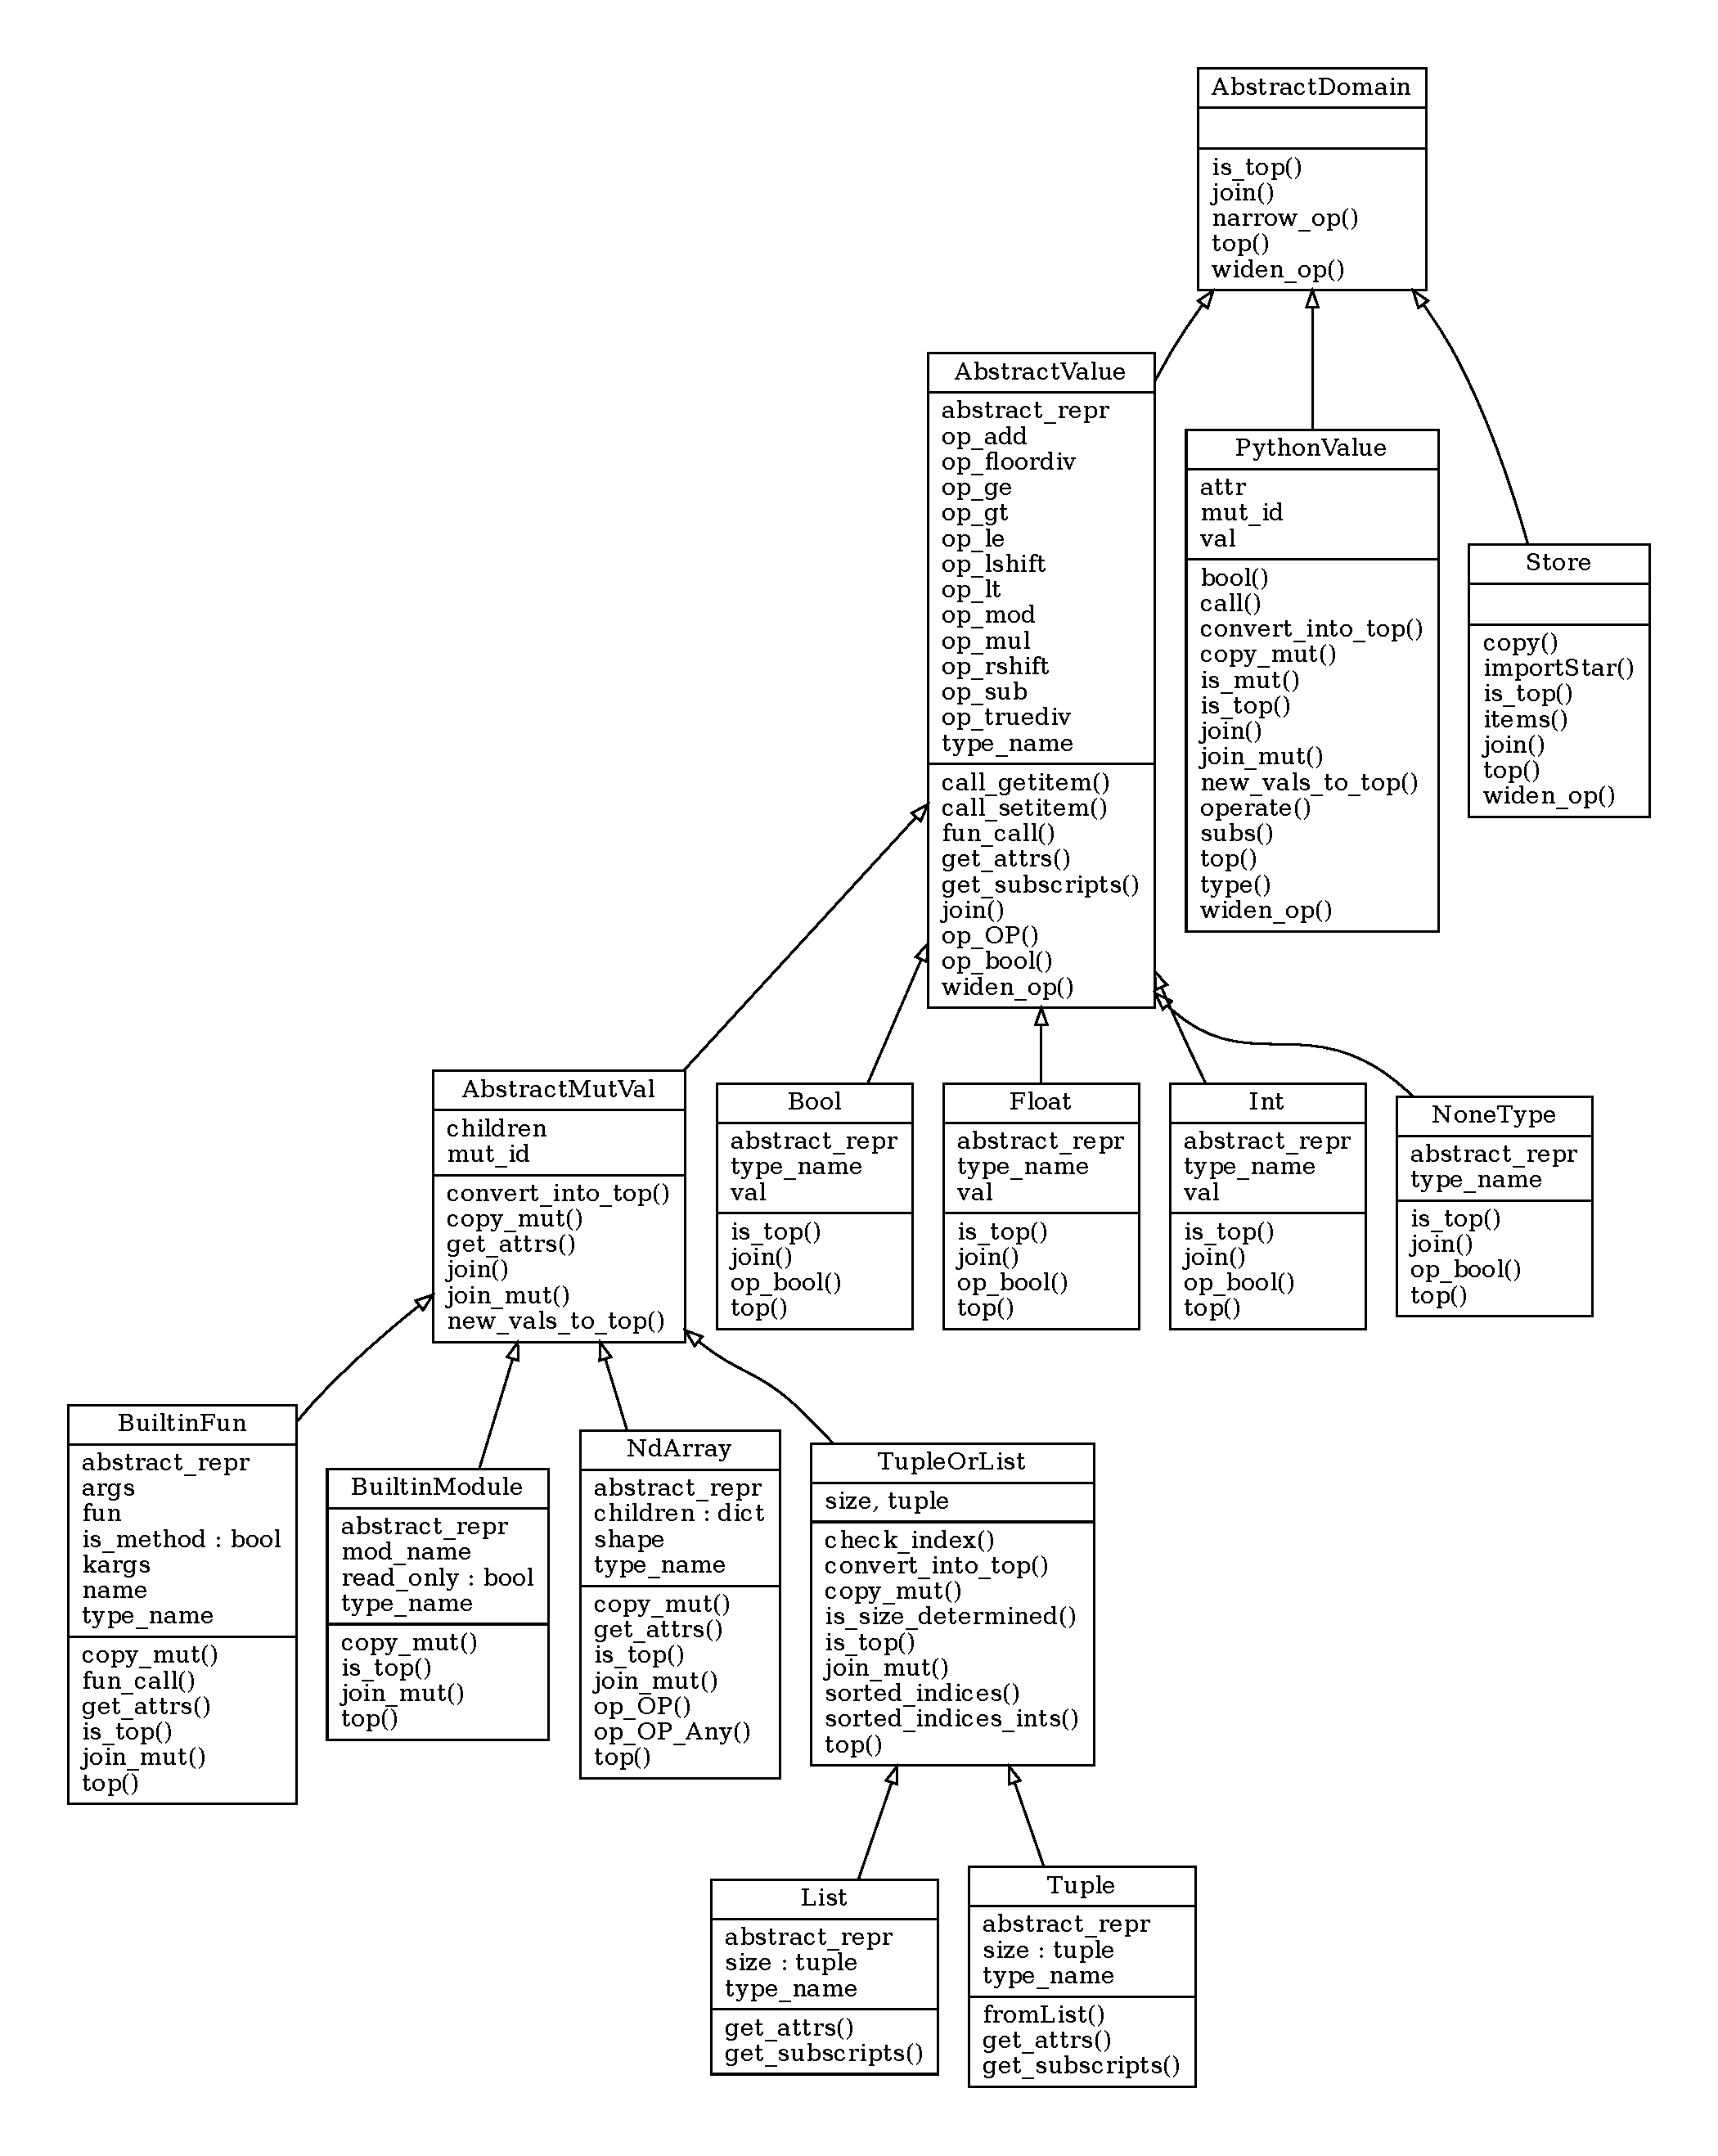
\includegraphics[width=0.9\textwidth,height=\textheight]{figures/classes_Pytropos-small.pdf}
{\todo{add types to each attribute, and add hidden attributes like
\texttt{\_\_getitem\_\_}}}

\texttt{\textless{}prim-callable\textgreater{}} and all other
\texttt{Objects\#} are implemented by a subclass of
\texttt{AbstractMutVal}: \texttt{\textless{}prim-callable\textgreater{}}
by \texttt{BuiltinFun}, \texttt{Module} objects by
\texttt{BuiltinModule}, \texttt{list}s by \texttt{List}, and
\texttt{tuple} by \texttt{Tuple}.

{\inlinetodo{mention that \texttt{children} is the function
\texttt{Key\ -\textgreater{}\ Addr\ +\ Undefined}}} {\inlinetodo{mention
that \texttt{joinVal} is defined as \texttt{join\_mut} in
\texttt{PythonValue}, and \texttt{joinObject} is defined as
\texttt{join\_mut} in \texttt{AbstractMutVal}}}

\hypertarget{validation-and-discussion}{%
\chapter{Validation and Discussion}\label{validation-and-discussion}}

{\ichange{This is just a DRAFT! REVISE!!}}

So, this chapter is about which kind of tests where performed and which
were considered but didn't cut it. The Python Regression tests are very
broad in scope, they use too many builtin capabilities which makes it
hard for a prototype like Pytropos to make any of them work (and that is
maybe why they are the regression tests for Python, after all they need
to check as many characteristics as possible!).

\hypertarget{validation}{%
\section{Validation}\label{validation}}

{\inlinetodo{Over which set of problems you tested your code. The
problems are pieces of code written by me on my own and other collected
from programs from the internet}}

I created two types of tests: unit regression tests and property-based
tests. The unit tests let us check for any kind of anomalous behaivour
while property-based tests ensure that the abstraction follows the
Python implementation that underlies.

Comparing against the official regression tests is left for future work,
as the number of builtin characteristics does not yet reach a
satisfactory level to check.

\hypertarget{unit-tests}{%
\subsection{Unit Tests}\label{unit-tests}}

There are a total of 79 unit tests checking various parts of the
Abstract Interpreter. The tests can be categorised into:

\begin{itemize}
\tightlist
\item
  binary operations
\item
  type annotations
\item
  numpy library
\item
  if branching
\item
  while looping
\item
  lists and tuples
\item
  join stores
\end{itemize}

In the table below the result of executing all tests can be seen. The
coverage is not 100\% as Pytropos is still in development. The tests
check not only for what Pytropos is able to do now, but what it should
be able given the description of it given in the document.

\begin{verbatim}
Category     Total lines    Tests     Time analysing   covered  non-covered   Total coverage
Binary ops   120            10        500ms            8        2             80%
\end{verbatim}

\hypertarget{property-based-tests}{%
\subsection{Property-based Tests}\label{property-based-tests}}

Property-based tests that try to disprove a property. For example, a
property of lists is that anytime you add a new element to a list of
size \texttt{n} you will get a list with size \texttt{n+1}. I use
property-based tests to check for correcness of Pytropos against Python
on builtin operations for builtin values.

There are a total of 20 of such tests. Because each one of them is a
property-based tests, they are tested against a 100 values that try to
disprove the property. This kind of testing proved to be extremely
helpful at the start of the development, as the \enquote{property-based
tester} was able to find numerous counter examples to the properties.
Python throws an exception on many cases of bad values, the
\enquote{tester} was able to reliably (at least at the start) to come up
with combinations of values that would go wrong when operated. Some of
the most honorable mentions are:

\begin{itemize}
\tightlist
\item
  Zero-division error on expressions like \texttt{5\ \%\ 0} or
  \texttt{5\ \%\ False}
\item
  Value error on expressions like \texttt{5\ \textless{}\textless{}\ -2}
\item
  Excesive High-memory consumption on expressions like
  \texttt{5\ \textless{}\textless{}\ 10**10}
\item
  Overflow error on expressions like \texttt{10**209\ +\ 2.0}
\end{itemize}

\hypertarget{discussion}{%
\section{Discussion}\label{discussion}}

Pytropos is still in a very young age. It is not able to check many,
many characteristics present in Python code (some of the biggest
culprits are \texttt{for} statement, custom classes and objects,
exception handling and the lack of builtin definitions), but when code
is given to it that it can actually check.

Pytropos is able to check for the many common cases and mistakes that
can be made when working with tensors. It is able to calculate the shape
of tensors in a variety of circumstances (NumPy's \texttt{array} can
evaluate almost anything as an array, therefore detecting the shape of
any value passed to \texttt{array} is an accomplishment in itself. An
example of why this is important can be seen in the library{\todo{add
ref to numpy mypy lib}}, where they define a stub for mypy to check of
the library numpy, and what they do in the case of \texttt{array} is
basically give up).

\hypertarget{related-work}{%
\chapter{Related Work}\label{related-work}}

{\ichange{Revise, rewrite and extend this subsection}}

A big, widely used, and mature language like Python has no lack of
Static Analysis tools. A big, widely used, and mature area like Machine
Learning has no lack of people trying to build tools to make writing
code for it easier. In this chapter, a brief overview of the many Static
Analysis tools developed for Python code and the several approaches
taken to solve the problem of tensor shapes.

\hypertarget{static-analysis-in-python}{%
\section{Static Analysis in Python}\label{static-analysis-in-python}}

{\inlinetodo{write down which are the possible classification categories
for Analysis Tools in Python}}

{\inlinetodo{add note in the difficulty of knowing what is the theory
behind some of the most widely used linters}}

The table below summarises the different tools and what they rely on:

\begin{verbatim}
Tool name/source |  Usage  | Analysis base  | Purpose                     |
---------------------------------------------------------------------------
@cannon.._2005   | Embeded | Type analysis  | Type checking               |
Pyflakes[ref]    | Linter  | NA             | Various checks              |
Pylint           | Linter  | NA             | Various checks              |
Pychecker        | Linter  | NA             | Various checks              |
MyPy             | Linter  | Type analysis  | Type checking               |
Enforce*+(defun) |         | Type analysis  | Type checking               |
Sagitta* (defun) |         | Type analysis  | Type checking               |
StyPy            | Linter  | Novel          | Type checking               |
Lyra             |         | AbstrInter     | Various analyses (including Value Analysis)   |
Pytropos         | Linter  | AbstrInter     | Value Analysis (specialised on tensor shapes) |
PyType           | Linter  |                | Type checking and inference |
ICBD (defun)     | Linter  |                | Type checking and inference |
Pyre             | Linter  | AbstrInter     | Type checking               |
Nagini           | Linter  | SMT (Viper)    | Verifier                    |
Typpete          | Linter  | SMT            | Type inference              |
fromherz...2018  | ?       | AbstrInter     | Value Analysis | Verifier   |
monat..2018      | ?       | AbstrInter     | Type Analysis               |
PyAnnotate*+     | Library | Type analysis  | Type inference              |

*: special cases, they are not an static analysis, but dynamic analysis!
?: tool has not been made public
+: uses gradual types

Pyflakes [@pyflakes2005]
Pylint [@thenaultpylint]
PyChecker [@norwitzpychecker]
Pytype https://github.com/google/pytype
ICBD https://github.com/kmod/icbd
Pyrecheck https://github.com/facebook/pyre-check
Sagitta https://github.com/peterhil/sagitta
Nagini https://github.com/marcoeilers/nagini (has paper)
Typpete https://github.com/caterinaurban/Typpete (two references, a thesis and a paper)
monat..2018 paper: Static Analysis by Abstract Interpretation Collecting Types of Python Programs
PyAnnotate https://github.com/dropbox/pyannotate
\end{verbatim}

{\inlinetodo{write a brief description of each one of the tools
presented in the table}}

{\inlinetodo{explain special case of the library \texttt{astroid} (part
of pylint), which is able to perform some Static Value Analysis. It
stops when it cannot determine the value of anything else. Pretty nice.
\texttt{astroid.extract\_node(\textquotesingle{}a=1\textbackslash{}nb=2\textbackslash{}nc=a+b\textbackslash{}nc\textquotesingle{});\ next(\_.infer())}.
https://astroid.readthedocs.io/en/latest/inference.html}}

{\inlinetodo{explain differences between lyra, fromherz..2018 and
Pytropos}}

{\inlinetodo{lyra was not the first to try abstract interpretation for
Python, mention pydrogen https://github.com/lapets/pydrogen}}

\hypertarget{tensor-shape-analysis}{%
\section{Tensor Shape Analysis}\label{tensor-shape-analysis}}

{\inlinetodo{add idea from http://nlp.seas.harvard.edu/NamedTensor
Alexander, who suggests building the libraries in a different way so we
do not have some of the problems of working with nameless shapes}}

{\inlinetodo{extend solutions described below with the new libraries you
found, comment below}}

\hypertarget{solutions-in-other-languages}{%
\subsection{Solutions in other
languages}\label{solutions-in-other-languages}}

We may think, If a type system is not expressive enough to capture the
shape of tensors, then we should just start writing code in a language
which does. We may write code in a language like Haskell or even C++,
which have very strong and expressive type systems (it is possible in
C++ to enforce the shape of the tensors with the use of templates and
constraints (C++20)).

In fact, solutions in other languages exists. For example,
\textcite{chen_typesafe_2017} type checks the shape of tensors
(operations) by restricting what can be constructed (via constraints in
the types of objects and functions). Chen's solution uses the powerful
type system of Scala (which runs over the JVM).
\textcite{eaton_statically_2006} does the same, although in an old
version of Haskell. Eaton's encoding of tensor shapes is awkward because
Haskell did not have, at the time, support for natural numbers at the
type level. Haskell also lacked on syntactic sugar for type functions.
\textcite{abe_simple_2015} implement type checking for matrices (aka,
tensors) in OCaml. The library detects the shape of the matrices at
compile time. \textcite{rakic_statically_2012} type check tensor shapes
(they call them matrices) with templates in C++. Templates are only
accessible at compile time, thus the Rakić et al.~library type checks at
compile.

One recent effort to type check tensor shapes in Haskell is the library
\texttt{tensorflow-haskell-deptyped} written by
\textcite{elkin_haskell_2018}. The library is written as a wrapper
around the library port of TensorFlow for Haskell.
\texttt{tensorflow-haskell-deptyped} enforces at the type level how and
which results a operation between compatible tensors is to be performed.

A different path to take is to extend an existing type checking system,
like MyPy, and extend it with dependent types. Dependent types allow us
to carry information from the term level to the type level, i.e.~we can
encode information of our data (available only at runtime) into the type
system. Over this extended type system, we could implement some
restrictions to the operations applied to different types (this is in
fact the strategy taken in the library tensorflow-haskell-deptyped).

\hypertarget{theoretical-solutions}{%
\subsection{Theoretical Solutions}\label{theoretical-solutions}}

The problem of mismatched shapes is not new, in fact, it is so common
that it has appeared several times with similar solutions
\autocites{arnold_specifying_2010}{griffioen_type_2015}{rink_modeling_2018}{slepak_array-oriented_2014}{trojahner_dependently_2009}.
All solutions, though, are theoretical, they propose type systems which,
if were to be implemented, could warranty type safety, i.e.~no
mismatching of tensor shapes could ever happen at runtime.

The following is a small discussion about the different solutions
proposed to type check tensors found in the literature\footnote{As a
  side note, it is interesting to notice how difficult is to communicate
  ideas in science. All the papers presented in this section hope to
  solve the same (or similar) problem, but they do not reference each
  other, which means that none of them knew what the others were doing.
  The principal reason for this, I think, it is because they all called
  the problem differently.}:

\begin{itemize}
\item
  \textcite{trojahner_dependently_2009}: A paper on type checking of
  arrays. They define all type restrictions using dependent types
  (something that no other paper does). The special keyword of this work
  is \enquote{array programming}.
\item
  \textcite{arnold_specifying_2010}: A paper focused on type checking of
  sparse \enquote{matrix} operations. They define a functional language
  that can be translated into a lower level language, or machine code.
  They give a complete formalization of the algorithms and proofs of
  correctness in Isabelle. The special keyword of this work is
  \enquote{sparse matrix}.
\item
  \textcite{griffioen_type_2015}: A paper focused in type checking and
  inference of arrays in array programming and vector spaces. They
  define a special type system in which tensors are first class
  citizens. The algorithm used for type checking is
  \enquote{Unification} which allows them to infer the type shape of
  arrays. The special keyword of this work is \enquote{array
  programming}.
\item
  \textcite{slepak_array-oriented_2014}: A paper that tries to formalise
  array-oriented programming languages and extend them with unit-aware
  operations. Array-oriented programming languages are languages which
  base all their computations in arrays (like matlab), but they usually
  aren't formalised. The types of arrays not only carry information
  about their shape but also of the unit they carry. The special
  keywords of this work are \enquote{array-oriented programming} and
  \enquote{unit-aware computation}.
\item
  \textcite{rink_modeling_2018}: In this paper, Rink formalises a type
  system to type check the shape of tensors and defines a language to
  use with the type system. It is a custom type system which does not
  require of dependent types. The special keyword of this work is
  \enquote{tensor manipulation language}.
\end{itemize}

\hypertarget{conclusions}{%
\chapter{Conclusions}\label{conclusions}}

{\ichange{This is just a DRAFT! REVISE!!}}

In this work I have presented the application of a very powerfull and
very well studied technique for Static Analysis (Abstract
Interpretation), applied to a domain where it has not been applied much
(just a couple of recent papers and applications are using it). In a
brief note the work done includes:

\begin{itemize}
\tightlist
\item
  A formalisation of a subset of Python 3.6
\item
  An Abstract Domain for Python Values
\item
  An Abstract Domain for Python program states
\item
  The semantics of an Abstract Interpreter for Python
\item
  The implementation of the Abstract Interpreter
\item
  A prove of concept domain where, tensor shapes, where the Abstract
  Interpreter could show its power
\item
  A series of tests showcasing the scenarios where the AI is able to
  work fine and show results
\item
  A way for developers to annotate code to improve the accuracy of the
  AI
\end{itemize}

The formalisation of the subset of Python showed one more attempt to
formalise the Python semantics. We focused on how this formalisation
could be used for a very specific library, the numpy library a corner
stone of modern Python.

To implement the Abstract Interpreter, we required the formalisation of
the Abstract Domain which carries the values stored in memory. The State
Abstract Domain is wholy defined by the join operation. The join
operation is the most complex piece in the whole work, it tries to
combine the information of two different states into one that contains
information from both. The values where they differ are then collapsed
properly to a \texttt{Top} value. \texttt{Top} values can be think of as
\texttt{?} types in Gradual Type systems, they are valid types/values
but carry only the information of their existance not what could be they
carrying.

Fortunately, the semantics of the Abstract Interpreter are not very
complicated, they just borrow their capabilities from the State Abstract
Domain and the semantics of Python. It is easy to see how the
formalisation could be extended to work with other values by just
augmenting the Abstract Domain.

\enquote{Extensive} testing showed that the implementation of the
Abstract Interpreter, Pytropos, is able to actually check many common
shape cases. The biggest problem of the implementation relies on the
lack of capabilities it can offer (harshly limited to forgo user-defined
functions and classes).

The Abstract Interpreter also lets itself to extend with type
annotations. Type Annotations are meant to be given by the user, who
always knows what is doing, and can tell the poor AI what the value of
some variable is. This is easily done by replacing the old value by the
new one with the annotation only if the annotation contains for
information about the variable than the value contained on it (ie, hint
\textless{} val).

\hypertarget{future-work}{%
\section{Future Work}\label{future-work}}

Python is a huge and rich language. The amount of Python characteristics
exceeds that of what a single human could try to implement for a work
like this. In fact, implementing an Abstract Interprer can be regarded
to be as hard, or harder, than a regular interpreter.

Much work left to do to try to match the power of Pytropos to make it
usable for the regular developer. I propose the following roadmap to
continue building the Abstract Interpreter:

\begin{itemize}
\tightlist
\item
  Extend Pytropos to include Exception handling (probably, a similar
  approach to that of {\todo{add ref to ai last year python}} could be
  applied here).
\item
  Improve how spliting stores and \textbf{join}ing them latter is
  done. The join operation between stores is very, very costly. It
  requires walking through both graphs/stores at the same time. That is
  extremely expensive when only a variable has changed its value between
  two different stores. This associated cost could be reduced if not a
  whole store is created everytime a new store is need to be created.
  (One way to do this is by using immutable structures for all values in
  the implementation. The current implementation uses the Heap provided
  by CPython underneat but if one where to define ones heap from scratch
  this would not be a problem).
\item
  Extend, again using the ideas put on the paper on ai {\todo{add ref,
  same as above}}, Pytropos to handle break statements.
\item
  Extend the definition of Store from a simple Global scope + heap to
  something that handles different levels of scope. This would allow an
  easier implementation of user defined functions. The function scope of
  Python is middly complex (this is due to the \texttt{compile}-ation
  process to which the parsed code is put to. Python does compile, but
  it does it very, very fast) with four different variable scopes:
  global, local, nonlocal, and class.
\item
  Once the interpreter handles user-defined functions properly,
  extending the interpreter to work with user-defined objects is not a
  big problem. The biggest difficulty is the inherit MRO behind the
  complex multi-classing system of Python.
\end{itemize}

{\inlinetodo{add idea that Pytropos could be run inside an IDE just as
paper: Sulir\_Poruban (2018) - Augmenting Source Code Lines with Sample
Variable Values}} {\inlinetodo{add idea that the parser could be
extended to add holes, or insert Top values, just as done in paper: Omar
et al (2018) - Live Functional Programming with Typed Holes (I wrote
something about it in the SoRI)}}

Besides what is left to do to make Pytropos more powerful, there are
some tasks related to the formality of the work. This work just
presented a formalisation of a subset of Python, an Abstract Domain for
Python, and \enquote{inferred} Abstract Semantics, but it nothing is
ever proved. I built from theories to make something workable, but it
may be good if we try to formalise a little bit more Python. We want
some warranties after all! The things that I consider should be done
next are:

\begin{itemize}
\tightlist
\item
  Give a complete and through formal definition for a subset of Python
  in a proof-assistant language such as Agda, Idris, Coq, Isabelle/HOL,
  or one of the many others.
\item
  Define in the same proof-assistance language the Abstract Domain, the
  properties it must follow, and the inferred semantics it produces.
\item
  Prove that the inferred semantics are in fact \textbf{inferred} from
  the Galois connection of the Abstract Domain.
\end{itemize}

Such a formalisation of Python would likely/hopefully help future
endeavours on proofs and verification.

Notice that any formalisation of Python must take some stance on how
closely it wants to follow the implementation of CPython. CPython has
many, many little undocumented semantic subtleties that trying to write
a full formal definition would probably defeat its purpose, namely, help
other projects where a clean and clear formalisation is necessary.

{\inlinetodo{expand on what you wrote in SoRI}}

\hypertarget{addendum-gotchas-and-other-ideas-to-static-analysis-in-python}{%
\chapter{Addendum: Gotchas and Other ideas to Static Analysis in
Python}\label{addendum-gotchas-and-other-ideas-to-static-analysis-in-python}}

{\ichange{This is just a DRAFT! REVISE!!}}

\emph{Note: This chapter is probably the most informal of the whole
book. The principal idea of this chapter is to explain a little bit
deeper the history of the whole thesis, some of the things I tried to
solve the problem at hand, and what avenues I found could be explored
and which are probably dead ends. This whole chapter is me rambling
about various stuff}

In here, I write on the multiple other ways I thought on how to
Statically analyse the shape of tensors. I explored some of them but
never really finish them, while others just proved to be bad ideas
altogether.

Some background. The principal, original, idea for my master thesis was
to check the shape of tensors and check the validity of tensor
operations. I did not consider Abstract Interpretation as my first
option to statically analyse code. In fact my whole exposure to Static
Analysis had been Type Inference, some Data Flow Analysis algorithms,
and some exposure into SMT solvers theory and practice.

I will mention each one of the approaches I tried in chronological
order.

{\nonsection{Tensor Shape Type Checking - Haskell}}

Everything started in Haskell. I wrote a wrapper library around a
Haskell wrapper library for TensorFlow \autocite{abadi_tensorflow_2016}.
The library uses one of the lastest additions to the language, Dependent
Types \autocite{eisenberg_dependent_2016}. Dependent Types allow me to
define the shape of tensors at the type level, which allows the compiler
to check for the correctness of tensor operations at compilation time.

My main motivation to use Haskell is its very strict type system, and
the tools that it incorporates to work with types. For example, in GHC,
the standard Haskell implementation, one can ask for the inferred type
of an expression by annotating the type with the type symbol
\texttt{\_}\footnote{They are called holes. There are two types of
  holes: (regular) holes and type holes. A hole is an unknown expression
  and a type hole is an unknown type. You can put a whole at the type
  level and the compiler will tell you what is the type that should be
  at that position. I found this incredibly neat and useful!}, thus we
can ask what shape of tensor should we use in the middle of an
operation.

Although, type checking tensor shapes in Haskell proved to be possible
and not all too hard, albeit a very verbose at times, I yet have to know
the first Deep Learning enthusiast who writes in Haskell. So, I decided
to apply the same idea into Python, the \enquote{language} of Deep
Learning.

Some efforts have been made to add type inference and type checking into
Python (See Related Work, Chapter \ref{related-work})), the most
important one being MyPy.

{\nonsection{Extending MyPy}}

MyPy builds on the idea of Gradual Typing. MyPy is able to infer the
type of primitive values and allows optional annotations to check the
code. Sadly, MyPy does not consider literal numbers as valid types
(\texttt{int}, \texttt{float}, \texttt{List{[}int{]}} are valid types
but no \texttt{3} or \texttt{List{[}2,\ int{]}}), so it is currently
impossible to type annotate a variable with the size of the variable,
e.g., something like \texttt{np.ndarray{[}2,\ 3,\ 4{]}}.

But hope is still not lost! We can encode numbers in MyPy's Type System
in a similar way to how was done in
\autocites{chen_typesafe_2017}{eaton_statically_2006}. We can encode 1
as \texttt{Tuple{[}None{]}}, 2 as \texttt{Tuple{[}None,\ None{]}}, and
so on.

Additionally, we can compare fields between two variables in an
operation with the use of \texttt{TypeVar}s (variables at the type
level). With these two ideas, we can rudimentary check the shapes of
tensors. First we write a stub file \autocite{pep484} with type
annotations to check for the shape of NumPy arrays:

\begin{Shaded}
\begin{Highlighting}[]
\CommentTok{# numpy.pyi}
\ImportTok{from}\NormalTok{ typing }\ImportTok{import}\NormalTok{ Any, Generic, Optional, Tuple, TypeVar}

\NormalTok{S }\OperatorTok{=}\NormalTok{ TypeVar(}\StringTok{'S'}\NormalTok{)  }\CommentTok{# Used for dtype}
\NormalTok{Shape }\OperatorTok{=}\NormalTok{ TypeVar(}\StringTok{'Shape'}\NormalTok{)  }\CommentTok{# Used for the shape}
\NormalTok{s1 }\OperatorTok{=}\NormalTok{ TypeVar(}\StringTok{'s1'}\NormalTok{)  }\CommentTok{# Another variable to use as reference to a shape}
\NormalTok{s2 }\OperatorTok{=}\NormalTok{ TypeVar(}\StringTok{'s2'}\NormalTok{)}
\NormalTok{s3 }\OperatorTok{=}\NormalTok{ TypeVar(}\StringTok{'s3'}\NormalTok{)}


\KeywordTok{class}\NormalTok{ ndarray(Generic[S, Shape]):}
    \KeywordTok{def} \FunctionTok{__init__}\NormalTok{(}\VariableTok{self}\NormalTok{, shape: Any) }\OperatorTok{->} \VariableTok{None}\NormalTok{: ...}

    \KeywordTok{def}\NormalTok{ dot(}
            \VariableTok{self}\NormalTok{: }\StringTok{'ndarray[S,Tuple[s1,s2]]'}\NormalTok{,}
\NormalTok{            b: }\StringTok{'ndarray[S,Tuple[s2,s3]]'}
\NormalTok{    ) }\OperatorTok{->} \StringTok{'ndarray[S,Tuple[s1,s3]]'}\NormalTok{: ...}

    \KeywordTok{def} \FunctionTok{__add__}\NormalTok{(}
            \VariableTok{self}\NormalTok{: }\StringTok{'ndarray[S,Shape]'}\NormalTok{,}
\NormalTok{            value: }\StringTok{'ndarray[S,Shape]'}
\NormalTok{    ) }\OperatorTok{->} \StringTok{'ndarray[S,Shape]'}\NormalTok{: ...}


\KeywordTok{def}\NormalTok{ array(}\BuiltInTok{object}\NormalTok{: Any) }\OperatorTok{->}\NormalTok{ ndarray[Any, Shape]: ...}
\end{Highlighting}
\end{Shaded}

And now we write the piece of code to type check:

\begin{Shaded}
\begin{Highlighting}[]
\ImportTok{import}\NormalTok{ numpy }\ImportTok{as}\NormalTok{ np}
\ImportTok{from}\NormalTok{ typing }\ImportTok{import}\NormalTok{ Tuple}

\NormalTok{one   }\OperatorTok{=}\NormalTok{ Tuple[}\VariableTok{None}\NormalTok{]}
\NormalTok{two   }\OperatorTok{=}\NormalTok{ Tuple[}\VariableTok{None}\NormalTok{, }\VariableTok{None}\NormalTok{]}
\NormalTok{three }\OperatorTok{=}\NormalTok{ Tuple[}\VariableTok{None}\NormalTok{, }\VariableTok{None}\NormalTok{, }\VariableTok{None}\NormalTok{]}
\NormalTok{four  }\OperatorTok{=}\NormalTok{ Tuple[}\VariableTok{None}\NormalTok{, }\VariableTok{None}\NormalTok{, }\VariableTok{None}\NormalTok{, }\VariableTok{None}\NormalTok{]}

\CommentTok{# x has shape (2,3)}
\NormalTok{x }\OperatorTok{=}\NormalTok{ np.array([[}\DecValTok{1}\NormalTok{, }\DecValTok{2}\NormalTok{, }\DecValTok{3}\NormalTok{], [}\DecValTok{4}\NormalTok{, }\DecValTok{5}\NormalTok{, }\DecValTok{6}\NormalTok{]])  }\CommentTok{# type: np.ndarray[float, Tuple[two, three]]}

\CommentTok{# y has shape (4,1)}
\NormalTok{y }\OperatorTok{=}\NormalTok{ np.array([[}\DecValTok{7}\NormalTok{], [}\DecValTok{0}\NormalTok{], [}\DecValTok{2}\NormalTok{], [}\DecValTok{1}\NormalTok{]])    }\CommentTok{# type: np.ndarray[float, Tuple[four, one]]}

\NormalTok{w }\OperatorTok{=}\NormalTok{ x }\OperatorTok{+}\NormalTok{ y  }\CommentTok{# fails! And MyPy warns us!! :D}

\CommentTok{# THIS SHOULD FAIL IN MYPY!! But it doesn't :(}
\NormalTok{z }\OperatorTok{=}\NormalTok{ x.dot(y)  }\CommentTok{# type: np.ndarray[float, Tuple[two, one]]}
\end{Highlighting}
\end{Shaded}

Everything seems to work perfectly, MyPy detects that the two numpy
arrays cannot be added together because the have different shapes, but
MyPy does not detect the error on multiplying two non-compatible
matrices. We told MyPy in the stub that the shape of the last dimension
in \texttt{self} (\texttt{s2}) should be the same as the first dimension
in \texttt{b}, but MyPy does not verify this condition
(\texttt{three\ !=\ four}).

Unfortunatelly, MyPy's \texttt{TypeVar}s are not fully-fledged type
variables. MyPy does not handle Dependent Types, so a solution as the
one suggested for Haskell could not completely be coded.

Two options came from this experiment, either look how to extend MyPy
type variables handling to work in the general case or ignore type
checking as a possible solution at the moment.

{\nonsection{StyPy}}

As I mentioned in Chapter \ref{pytropos-analysis-implementation}, before
I encountered Abstract Interpretation as a way to Statically Analyse
code\footnote{I know, it is a very old, well understood, and broadly
  applied analysis technique but I didn't know much about the broad
  world of Static Analysis before I delved deep into it.} I found
\emph{StyPy} \autocite{ortin_towards_2015}.

The idea behind StyPy is to reuse the infraestructure of the language to
analyse to not write everything from scratch. The idea is to take the
code to analyse and rewrite/transform it into a new piece of code that
when run it performs Static Type Analysis. This approach presents to
difficulties: first, it was planned as a technique for Static Type
Analysis not Static Value Analysis, and second, it is a very naïve and
novel idea, it is not very well formalised.

When you require to know only the type of a variable, its value becomes
irrelevant. If we do not consider any weird introspection Python
capabilities, it does not matter how many times you run a loop a
variable will always keep the same type after the first loop iteration,
i.e.~there is no need to consider complex scenarios and joining
operations for the type of a variable as we need to consider for the
value of a variable inside a loop.

There have not been any updates on the theory behind the project since
the paper was published in 2015.

All in all, the idea of reusing some of the infraestructure by rewriting
the code and running it in the same platform where one wants to analyse
the code is a very interesting idea. In fact, this idea has been applied
in other static analyses, for example, \textcite{lauko_symbolic_2018}
explain how they built a symbolic analyser for LLVM bytecode by reusing
some of the infraestructure of LLVM and not rewriting a complete
interpreter for LLVM from the ground up.

Pytropos started from the same idea of StyPy, transform and run modified
code. The idea would be that any variable in the (extended) interpreter
could be any of Python's or \texttt{Any} (\texttt{?}, the special type
introduced in Gradual Typing). An \texttt{Any} value would tell me that
I have no idea of the value contained in the variable, just that the
variable contains a variable. I discarded the idea of modifying StyPy as
it would mean rewriting the whole program for my purpose. So I went on
looking different projects that I could modify to implement the Static
Value Analysis I was considering.

{\nonsection{Modify PyPy}}

Once I considered building a special purpose interpreter to analyse the
shape of tensors (as an Abstract Interpreter is), I took a look in other
projects that had implemented interpreters for python. a very
interesting project is pypy. pypy \autocite{krekel_pypy_2007} is a
project focused on providing an alternative implementation of python
with added characteristics. most importantly, pypy is written in python
(or a subset of python, called rpython) and pypy can be extended/its
semantics can be modified. apparently, pypy offers a way to change the
semantics of the interpreter\footnote{the object space can be modified
  as explained in \url{http://doc.pypy.org/en/latest/objspace.html}}.

both characteristics; pypy being written in python, allowing for an easy
introspection and modification of its internals, and the ease of
modifing some of its semantics; made me think of using pypy as a
\enquote{base} for the custom made interpreter. i did not follow this
route because the work to be done to allow having different states of a
program and joining them (used in \texttt{if} branching when choice can
be made between two branches) seemed to require rewritting a big chunk
of the core of pypy. starting from zero seemed a better idea.

{\nonsection{abstract interpretation}}

in the end, i decided to build my own interpreter from scratch. it took
me a couple of months to arrive to something relatively usable but i
found out in the process that branching, loops, exceptions, and breaking
control statements made the implementation of a interpreter that used
\texttt{any} values very challenging (how are the semantics of a
non-deterministic \texttt{if}, of a loop, an exception, etc).

it became clear that trying to build an (extended) interpreter from
scratch would be very hard if no clear formal framework was used to put
everything into perspective. enter abstract interpretation. i cannot say
that i found abstract interpretation as the solution for the many
problems that an extended value \enquote{system} presented, because i
had no idea such thing existed.

as you may have noticed, i just arrived a the \enquote{proposed}
solution of my problem (static value analysis) by \enquote{mere} chance.
i was looking at the literature of static analysis, but i thought there
was little i could use from it. how wrong was i! always so
smartass{\todo{change wording}}.

anyway, once i studied together with my advisors the theory of abstract
interpretation, i knew that ai was the solution for my problem. it was a
long path nontheless, as it required to formalise a couple of things
about the language and define an abstract domain for the state of the
language, which proved to be challenging but rewarding.

now, i must mention here that i did came across a project that was doing
pretty much what i wanted to do, namely an abstract interpreter for
python. {\todo{add ref to lyra}} lyra is a project led by {\todo{fill
me}} which purpose is to build an abstract interpreter for python. there
are two reasons why i chosed not to use lyra for this thesis: the first
is purely egothistical and not practical at all, i wanted to build
something from my own, something from \enquote{scratch}\footnote{please,
  dear advisors, do not kill me for writing this!}; the second reason
was that i had found the idea of reusing some of the python
infraestructure too fascinating to let it into oblivion, rewriting
python code to run it into with python seems just a nice metaidea.

{\nonsection{Other Ideas}}

Other routes, I did considered to follow but did not because of time
restrictions where:

\begin{itemize}
\tightlist
\item
  If all we wanted was to check the shape of tensors and tensor
  operations for a couple of scenarios, we could build a Static Analysis
  out of various Data Flow Algorithms. Data flow analyses are simple,
  well studied, and already implemented in a couple of Static Analysis
  frameworks {\todo{add reference to an Overview of Program Analysis
  framework that the mention (I think it was for Netbeans or some other
  IDE)}}. The only work would be combining them adecuately to know the
  shape of tensors and consequently check for the correctness of a
  couple of cases.
\item
  Another option may have been encoding the shapes as constraints. The
  constraints could be checked using an out of the shelve equation
  solver (SMTs). In fact, a big chunk of the work for this has already
  been done, an implementation for Python for example {\todo{Add
  reference on ETH people doing this}}.
\end{itemize}

%----------------------------------------------------------------------------------------
%	THESIS CONTENT - APPENDICES
%----------------------------------------------------------------------------------------

%\appendix % Cue to tell LaTeX that the following "chapters" are Appendices

% Include the appendices of the thesis as separate files from the Appendices folder
% Uncomment the lines as you write the Appendices

%\include{Appendices/AppendixA}
%\include{Appendices/AppendixB}
%\include{Appendices/AppendixC}

%----------------------------------------------------------------------------------------
%	BIBLIOGRAPHY
%----------------------------------------------------------------------------------------

\printbibliography[heading=bibintoc]

%----------------------------------------------------------------------------------------

\end{document}
